% !TEX TS-program = pdflatex
% !TEX encoding = UTF-8 Unicode

% This is a simple template for a LaTeX document using the "article" class.
% See "book", "report", "letter" for other types of document.

\documentclass[12pt]{article} % use larger type; default would be 10pt
\usepackage[fontsize=12pt]{fontsize}
\renewcommand{\baselinestretch}{1.5} % linespacing=1.5
\usepackage[T2A]{fontenc} % кодировка
\usepackage{fontspec} % for changing fonts 
% \setmainfont{Times New Roman}
\setmainfont{Minion Pro}
% \setmainfont{Roboto}
% \usepackage[utf8]{inputenc} % set input encoding (not needed with XeLaTeX)
\usepackage[english]{babel} % for cyrillic letters support
\usepackage[parfill]{parskip} % remove space vefore parapraph
\setlength{\parskip}{0pt} % additional skip between paragraphs


%%% PAGE DIMENSIONS
\usepackage{geometry} % to change the page dimensions
\geometry{a4paper} % or letterpaper (US) or a5paper or....
\geometry{left=30mm,right=20mm,top=15mm, bottom=15mm} % for example, change the margins to 2 inches all round
% \graphicspath{{./images/}}
% \geometry{landscape} % set up the page for landscape
%   read geometry.pdf for detailed page layout information

\usepackage{graphicx} % support the \includegraphics command and options

% \usepackage[parfill]{parskip} % Activate to begin paragraphs with an empty line rather than an indent

%%% PACKAGES
\usepackage{blindtext}
\usepackage{booktabs} % for much better looking tables
\usepackage{multirow}
\usepackage{array} % for better arrays (eg matrices) in maths
\usepackage{paralist} % very flexible & customisable lists (eg. enumerate/itemize, etc.)
\usepackage{verbatim} % adds environment for commenting out blocks of text & for better verbatim
\usepackage{subfig} % make it possible to include more than one captioned figure/table in a single float
\usepackage{cmap} % search in pdf
\usepackage{longtable} % for long tables 
\usepackage{lscape}
\usepackage{hyperref} % for hyperlinks
\usepackage{listings} % for code listings
% These packages are all incorporated in the memoir class to one degree or another...

%% Useful packages
\usepackage[colorinlistoftodos]{todonotes}
% \usepackage[colorlinks=true, allcolors=blue]{hyperref}



\usepackage{amsmath,amsthm,amsfonts,amssymb,amscd, fancyhdr, color, comment, graphicx, environ}
\usepackage{float}
\usepackage{mathrsfs}
\usepackage[math-style=ISO]{unicode-math}
\setmathfont{TeX Gyre Termes Math}
\setmonofont{Hack Nerd Font Mono}
\usepackage{lastpage}
\usepackage[dvipsnames]{xcolor}
% \usepackage[framemethod=TikZ]{mdframed}
\usepackage{indentfirst}
\usepackage{thmtools}
\usepackage{shadethm}
\usepackage{setspace}


\definecolor{codegreen}{rgb}{0,0.6,0}
\definecolor{codegray}{rgb}{0.5,0.5,0.5}
\definecolor{codepurple}{rgb}{0.58,0,0.82}
\definecolor{backcolour}{rgb}{0.95,0.95,0.92}


%%% HEADERS & FOOTERS
\usepackage{fancyhdr} % This should be set AFTER setting up the page geometry
\pagestyle{fancy} % options: empty , plain , fancy
\renewcommand{\headrulewidth}{0pt} % customise the layout...
\lhead{}\chead{}\rhead{}
\lfoot{}\cfoot{\thepage}\rfoot{}

%%% SECTION TITLE APPEARANCE
\usepackage{titlesec}
\usepackage{sectsty}
\sectionfont{\centering}
\subsectionfont{\centering}

\usepackage{enumitem}
\setlist{nolistsep}

\hypersetup{
    colorlinks=true,
    linkcolor=black,
    filecolor=magenta,      
    urlcolor=blue,
    pdftitle={Overleaf Example},
    pdfpagemode=FullScreen,
    }
\urlstyle{same}




\lstdefinestyle{mystyle}{
    extendedchars=\true,
    inputencoding=utf8x,
    backgroundcolor=\color{backcolour},   
    commentstyle=\color{codegreen},
    keywordstyle=\color{magenta},
    numberstyle=\tiny\color{codegray},
    stringstyle=\color{codepurple},
    basicstyle=\ttfamily\footnotesize,
    breakatwhitespace=false,         
    breaklines=true,                 
    captionpos=b,                    
    keepspaces=true,                 
    numbers=left,                    
    numbersep=5pt,                  
    showspaces=false,                
    showstringspaces=false,
    showtabs=false,                  
    tabsize=2
}

\lstset{style=mystyle}




% \allsectionsfont{\sffamily\mdseries\upshape} % (See the fntguide.pdf for font help)
% (This matches ConTeXt defaults)

%%% ToC (table of contents) APPEARANCE
% \usepackage[nottoc,notlof,notlot]{tocbibind} % Put the bibliography in the ToC
% \usepackage[titles,subfigure]{tocloft} % Alter the style of the Table of Contents
% \renewcommand{\cftsecfont}{\rmfamily\mdseries\upshape}
% \renewcommand{\cftsecpagefont}{\rmfamily\mdseries\upshape} % No bold!
\makeatletter
\renewcommand{\fnum@figure}{Picture. \thefigure}
\makeatother



\renewcommand\lstlistingname{Algorithm}
\renewcommand\lstlistlistingname{Algorithms}
\def\lstlistingautorefname{Alg.}


\title{Анализ и сравнение алгоритмов сортировки}
\author{Бактыбеков Н.Б.}

\begin{document}
\begin{titlepage}

\newcommand{\HRule}{\rule{\linewidth}{0.5mm}} % Defines a new command for the horizontal lines, change thickness here

%----------------------------------------------------------------------------------------
%	LOGO SECTION
%----------------------------------------------------------------------------------------
\centering

\includegraphics[width=8cm]{title/logo_inai.jpg}\\[1cm] % Include a department/university logo - this will require the graphicx package
 
%----------------------------------------------------------------------------------------

\center % Center everything on the page

%----------------------------------------------------------------------------------------
%	HEADING SECTIONS
%----------------------------------------------------------------------------------------

\textsc{\LARGE СРСП}\\[1.5cm] 
\textsc{\Large }\\[0.5cm] 
\textsc{\large WIN-1-22}\\[0.5cm] 

%----------------------------------------------------------------------------------------
%	TITLE SECTION
%----------------------------------------------------------------------------------------
\makeatletter
\HRule \\[0.4cm]
{ \huge \bfseries \@title}\\[0.4cm] % Title of your document
\HRule \\[6.5cm]
 
%----------------------------------------------------------------------------------------
%	AUTHOR SECTION
%----------------------------------------------------------------------------------------

\begin{minipage}{0.4\textwidth}
\begin{flushleft} \large
\emph{Выполнил:}\\
\@author % Your name



\end{flushleft}
\end{minipage}
~
\begin{minipage}{0.4\textwidth}
\begin{flushright} \large
\emph{Проверил:} \\
Картанова А.Д.\\[1.2em] 
\end{flushright}
\end{minipage}\\[2cm]
\makeatother

%----------------------------------------------------------------------------------------
%	DATE SECTION
%----------------------------------------------------------------------------------------

{\large \today}\\[2cm] % Date, change the \today to a set date if you want to be precise

\vfill % Fill the rest of the page with whitespace

\end{titlepage}


% \maketitle

\newpage
\tableofcontents{}
\setcounter{page}{1}

\newpage
\addcontentsline{toc}{section}{Индивидуальное задание}


\section*{Индивидуальное задание}

Решить 3 задачи

\textbf{Задача 1}

Удалить из массива элемент, расположенный после максимального элемента. Если удаление элемента невозможно, выдать об этом сообщение.



\textbf{Задача 2}

Вставить заданное значение после каждого элемента массива, расположенного до первого нулевого элемента. Если вставка элементов невозможна, выдать об этом сообщение.



\textbf{Задача 3}

Реализовать алгоритм трех методов сортировки:

\begin{enumerate}
    \item Сортировка Бэтчера
    \item Сортировка на основе приоритетных очередей
    \item Сортировка Пирамидой
\end{enumerate}

Сравнить эти три сортировки по критериям:

\begin{enumerate}
    \item Скорость выполнения
    \item Потребление памяти
\end{enumerate}

Решить каждую задачу в отдельной программе. Реализовать программу средствами языка программирования Python.






\section{Задача 1}
\subsection{Условие задачи}

Удалить из массива элемент, расположенный после максимального элемента. Если удаление элемента невозможно, выдать об этом сообщение.

\subsection{Постановка задачи}
\textbf{Входные данные:}

arr - массив из N элементов.

\textbf{Выходные данные:}

arr - результирующий массив из N-1 элементов.

\textbf{Условия и ограничения:}

Задание не может быть выполнено, если в массиве последний элемент является минимальным.



\subsection{Описание алгоритма}

Алгоритм задачи 1 описан в следующей блок-схеме:

\begin{figure}[H]
    \centering
    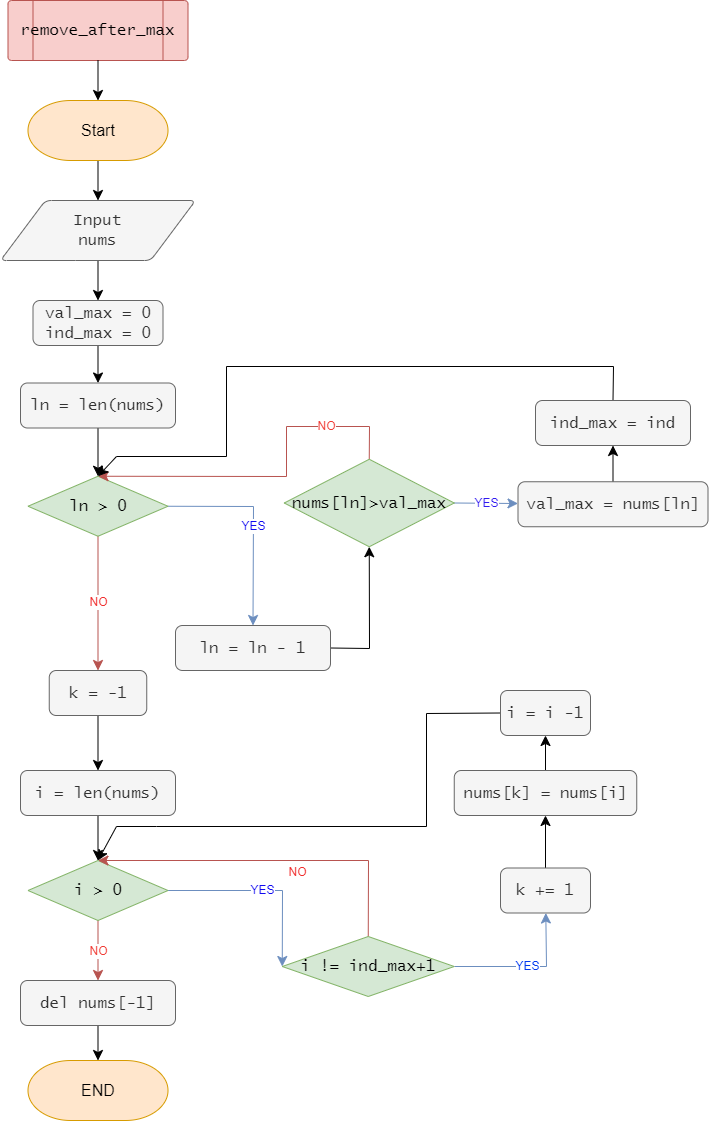
\includegraphics[width=0.8\textwidth]{./flowcharts/first_task.drawio.png}
    \caption{Блок схема Задание 1}
\end{figure}


\subsection{Контрольные примеры}
\begin{enumerate}
    \item a=[1, 5, 6, 2, 3, 4, 5, 9, 6, 7, 8]\\ new a=[1, 5, 6, 2, 3, 4, 5, 9, 7, 8]
    \item b=[8, 3, 6, 2, 3, 4, 5, 9, 3, 7, 2]\\ new b=[8, 3, 6, 2, 3, 4, 5, 9, 7, 2]
    \item Максимальный последний \\ c=[3, 8, 2, 7, 3, 5, 4, 1, 2, 0, 9]\\ new c=[3, 8, 2, 7, 3, 5, 4, 1, 2, 0, 9]
\end{enumerate}


\subsection{Реализация решения задачи}

Реализация задачи 1 оформлена ввиде функции в программе first-task.py


\subsection{Исходный код программы}

\lstinputlisting[language = python]{../two_tasks/first.py}

\subsection{Результаты работы программы}

\begin{figure}[H]
    \centering
    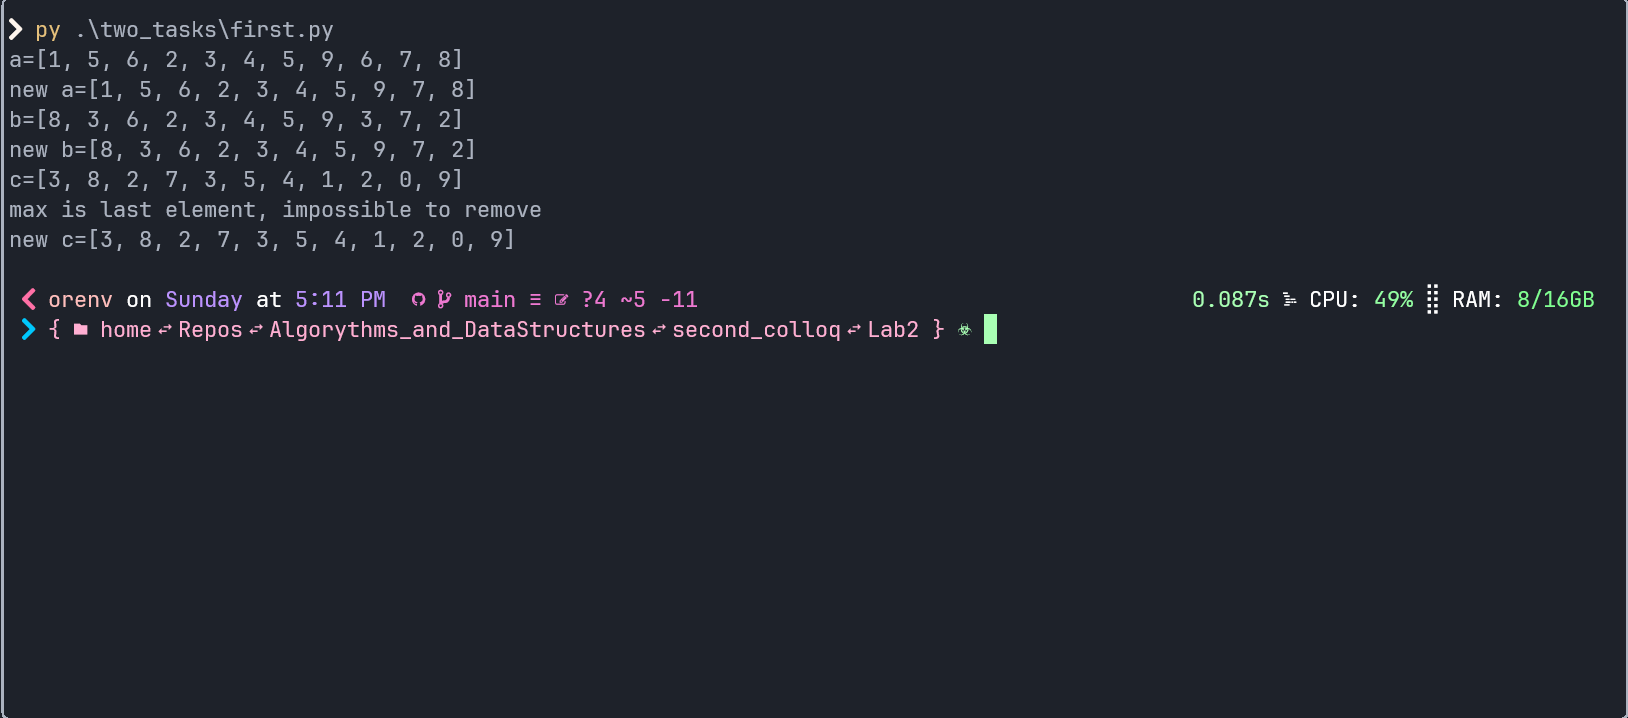
\includegraphics[width=0.8\textwidth]{./flowcharts/first_task.png}
    \caption{Блок схема Задание 1}
\end{figure}























\section{Задача 2}


\subsection{Условие задачи}

Вставить заданное значение после каждого элемента массива, расположенного до первого нулевого элемента. Если вставка элементов невозможна, выдать об этом сообщение.

\subsection{Постановка задачи}
\textbf{Входные данные:}

arr - массив из N элементов.
val - число которое нужно вставить

\textbf{Выходные данные:}

arr - результирующий массив из N+индекс-нуля элементов.

\textbf{Условия и ограничения:}

Задание не может быть выполнено, если в массиве первый элемент является нулевым.



\subsection{Описание алгоритма}

Алгоритм задачи 2 описан в следующей блок-схеме:

\begin{figure}[H]
    \centering
    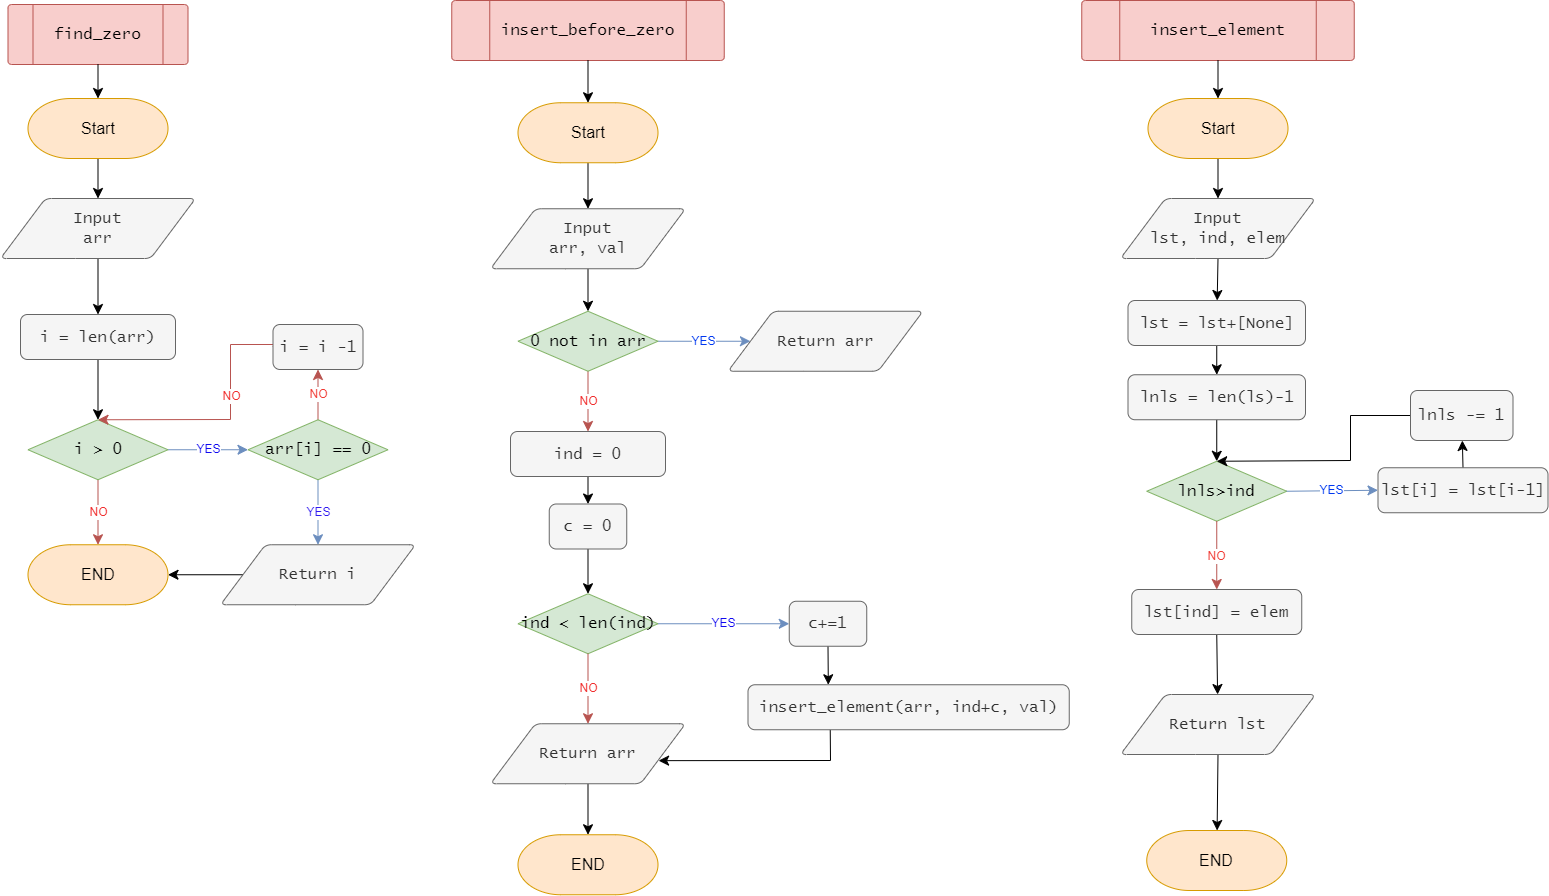
\includegraphics[width=0.8\textwidth]{./flowcharts/second_task.drawio.png}
    \caption{Блок схема Задание 2}
\end{figure}


\subsection{Контрольные примеры}
\begin{enumerate}
    \item a=[1, 5, 6, 0, 3, 4, 5, 9, 6, 7, 8] \\ new a=[1, 10, 5, 10, 6, 10, 0, 3, 4, 5, 9, 6, 7, 8]                                                                        
    \item b=[8, 3, 6, 2, 3, 4, 5, 0, 3, 7, 2] \\ new b=[8, 10, 3, 10, 6, 10, 2, 10, 3, 10, 4, 10, 5, 10, 0, 3, 7, 2]
    \item Первый элемент = 0 \\ c=[0, 8, 2, 7, 3, 5, 4, 1, 2, 0, 9] \\ new c=[0, 8, 2, 7, 3, 5, 4, 1, 2, 0, 9]

\end{enumerate}


\subsection{Реализация решения задачи}

Реализация задачи 2 оформлена ввиде функции в программе second-task.py


\subsection{Исходный код программы}

\lstinputlisting[language = python]{../two_tasks/second.py}

\subsection{Результаты работы программы}

\begin{figure}[H]
    \centering
    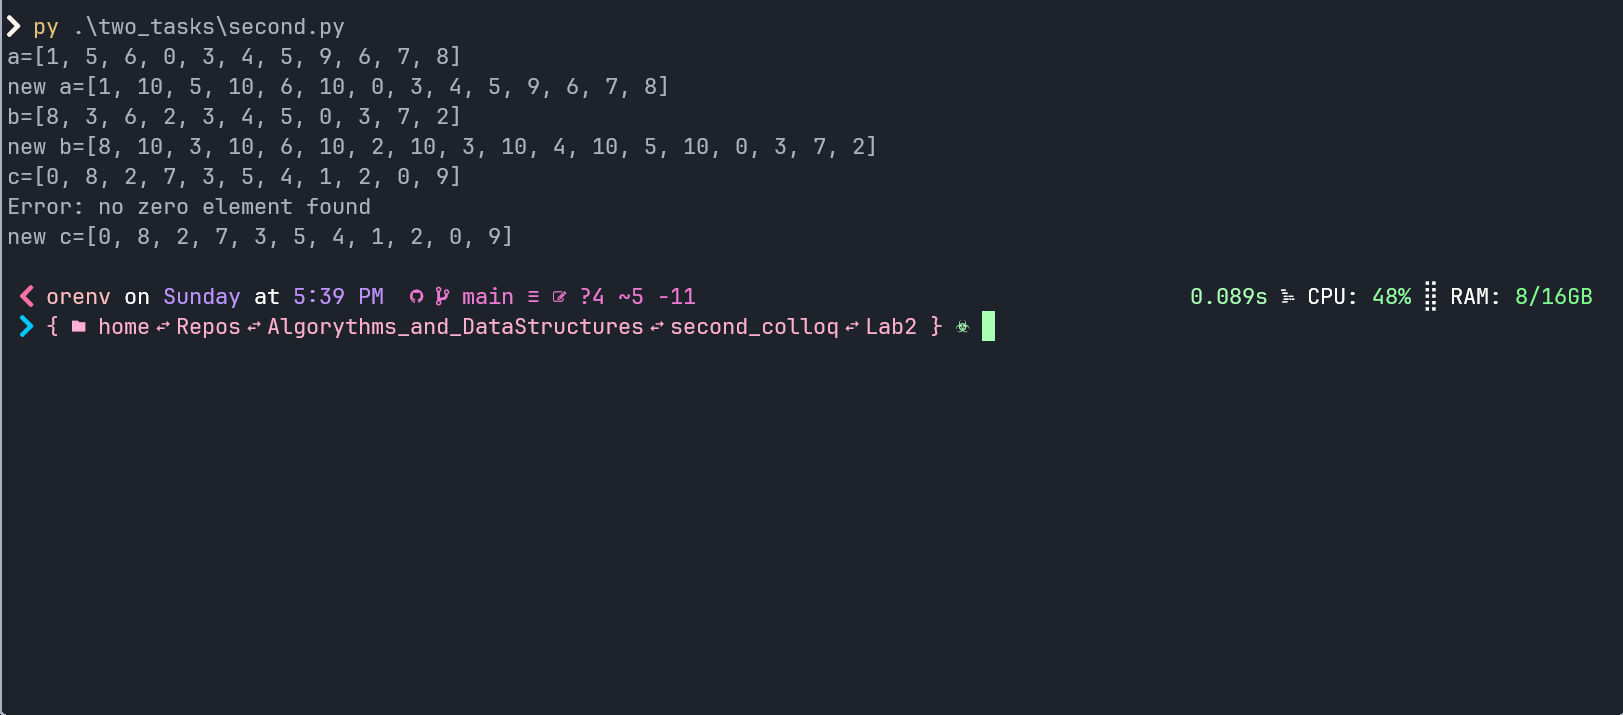
\includegraphics[width=0.8\textwidth]{./flowcharts/second_task.png}
    \caption{Запуск программы Задание 2}
\end{figure}




















\section{Задача 3}

\subsection{Условие задачи}


Реализовать алгоритм трех методов сортировки:

\begin{enumerate}
    \item Сортировка Бэтчера
    \item Сортировка на основе приоритетных очередей
    \item Сортировка Пирамидой
\end{enumerate}

Сравнить эти три сортировки по критериям:

\begin{enumerate}
    \item Скорость выполнения
    \item Потребление памяти
\end{enumerate}

Решить каждую задачу в отдельной программе. Реализовать программу средствами языка программирования Python.

\subsection{Постановка задачи}

\textbf{Входные данные:}

arr – cписок типа list, заполненный случайным образом

\textbf{Выходные данные:}
V – Скорость выполнения
M – Максимум расходуемой памяти
arr – отсортированный список


\subsection{Описание алгоритмов}

\textbf{Блок-схема подпрограммы сортировки Бэтчера:}



\begin{figure}[H]
    \centering
    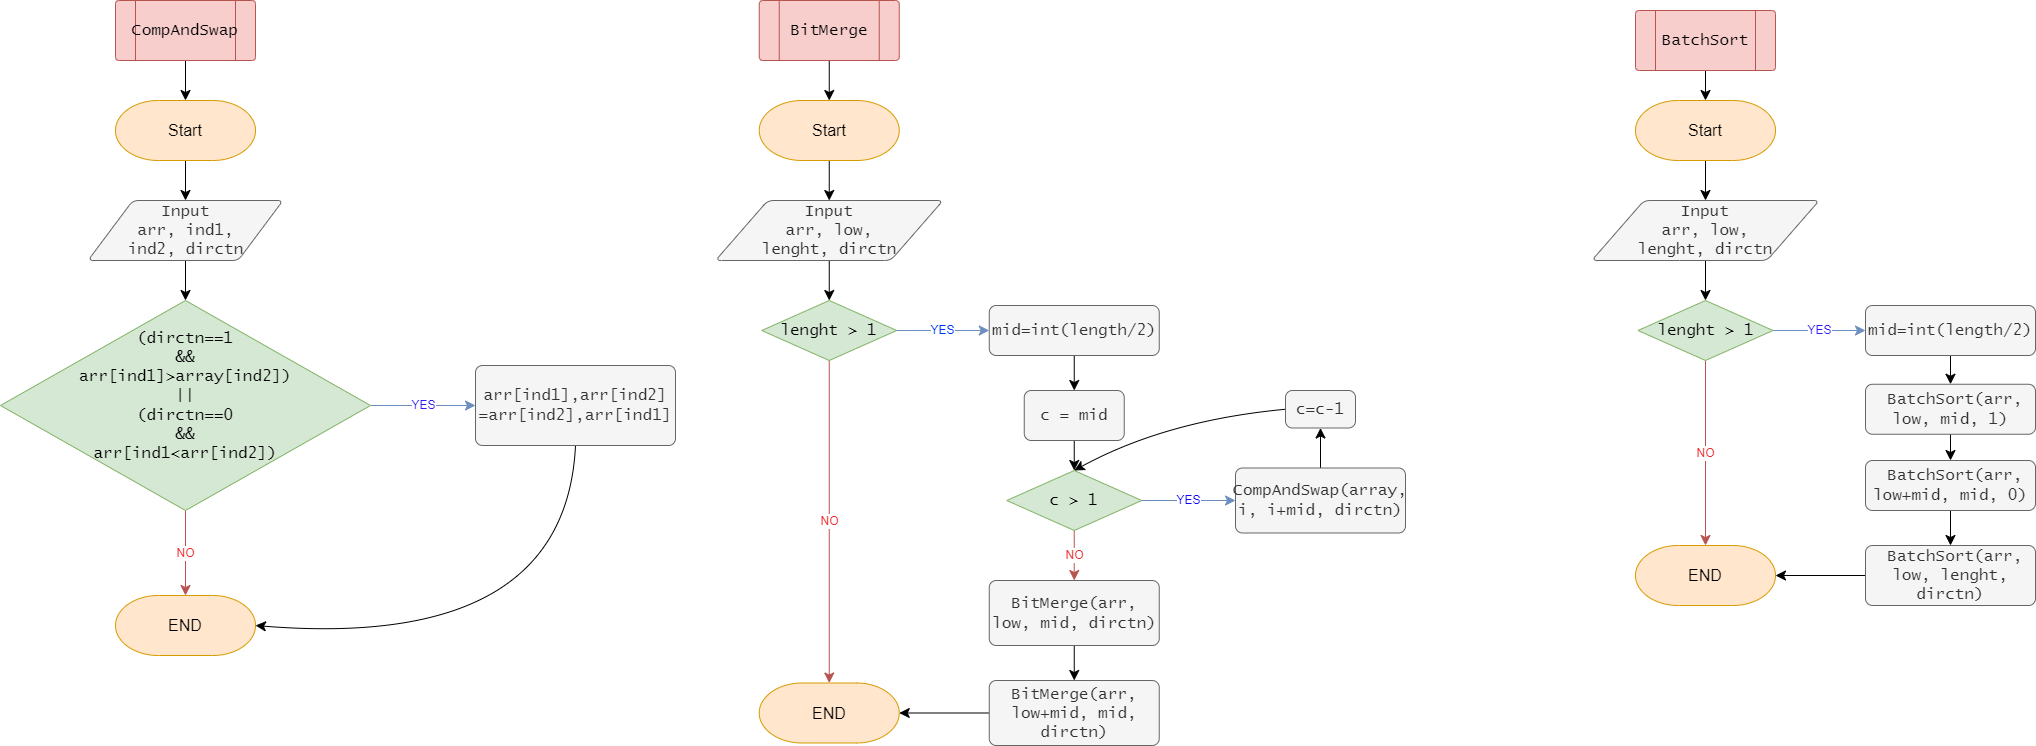
\includegraphics[width=1\textwidth]{./flowcharts/barcher.drawio.png}
    \caption{Сортировка Бэтчера}
\end{figure}


\textbf{Код программы с сортировкой Бэтчера}
\lstinputlisting[language = python]{../methods/batcher.py}




\textbf{Блок-схема подпрограммы сортировки Приоритетных очередей:}




\begin{figure}[H]
    \centering
    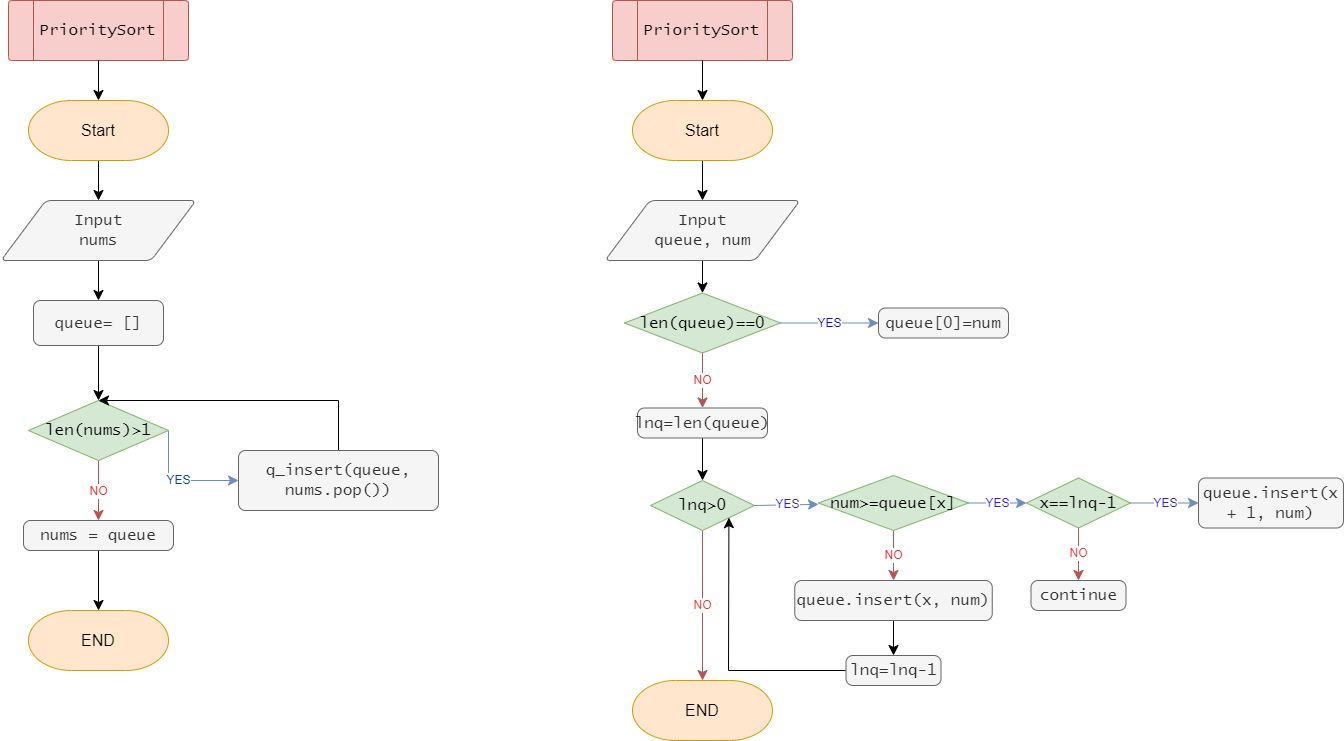
\includegraphics[width=1\textwidth]{./flowcharts/priority.drawio.png}
    \caption{Сортировка на основе Приоритетных очередей}
\end{figure}

\textbf{Код программы с сортировкой на основе Приоритетных очередей}
\lstinputlisting[language = python]{../methods/priority_func.py}



% \newpage
\textbf{Блок-схема подпрограммы сортировки Пирамидой:}



\begin{figure}[H]
    \centering
    \includegraphics[width=0.8\textwidth]{./flowcharts/pyramid.drawio.png}
    \caption{Запуск программы Задание 2}
\end{figure}

\textbf{Код программы с сортировкой Пирамидой}
\lstinputlisting[language = python]{../methods/pyramid.py}



\subsection{Контрольные примеры}
\textbf{Входные данные:}
ls: list[list[int]] список содержащий списки длиной 128 содержащие числа

\textbf{Выходные данные}
отсортированный массив, скорость выполнения, потребление памяти



\subsection{Реализация решения задачи}

Решение задачи 3 оформлено в виде трех программ: table.py, main.py, memory-usege.py. Программы используют три подпрограммы для выполнения сортировки: batcher-sort, priority-sort, pyramid-sort.


\subsection{Построение таблицы}


Программа 1 импортирует 3 подпрограммы сортировки и строит таблицу значений скорости и потребления памяти для трех алгоритмов сортировки

\textbf{Исходный код Программы 1}

\lstinputlisting[language = python]{../tables.py}


\textbf{Таким образом были построены таблицы:}


\begin{table}[H]\centering\caption{batcher sort}\begin{tabular}{|c|c|c|}\hline Запуск программы & Скорость выполнения   & Потребление памяти \\ \hline 1                & 0.0008890000026440248 & 20086784           \\ \hline 2                & 0.0008505000005243346 & 20086784           \\ \hline 3                & 0.0008888000011211261 & 20086784           \\ \hline 4                & 0.0008426999993389472 & 20086784           \\ \hline 5                & 0.0008421999955317006 & 20086784           \\ \hline 6                & 0.0008430000016232952 & 20086784           \\ \hline 7                & 0.0008448000007774681 & 20086784           \\ \hline 8                & 0.0008440000092377886 & 20086784           \\ \hline 9                & 0.0008452999900327995 & 20086784           \\ \hline 10               & 0.0008441999962087721 & 20086784           \\ \hline 11               & 0.0008420999947702512 & 20086784           \\ \hline 12               & 0.0008587999909650534 & 20086784           \\ \hline 13               & 0.000836799998069182  & 20086784           \\ \hline 14               & 0.0008390000002691522 & 20086784           \\ \hline 15               & 0.0008393000025535002 & 20086784           \\ \hline 16               & 0.0008424000116065145 & 20086784           \\ \hline 17               & 0.0008411999879172072 & 20086784           \\ \hline 18               & 0.0008405999979004264 & 20090880           \\ \hline 19               & 0.0008417999924859032 & 20090880           \\ \hline 20               & 0.0008437000069534406 & 20090880           \\ \hline 21               & 0.0008435000054305419 & 20090880           \\ \hline 22               & 0.0008436999924015254 & 20090880           \\ \hline 23               & 0.0008428000001003966 & 20090880           \\ \hline 24               & 0.0008422000100836158 & 20090880           \\ \hline 25               & 0.0008414000039920211 & 20090880           \\ \hline 26               & 0.0008418999932473525 & 20090880           \\ \hline 27               & 0.0008421999955317006 & 20090880           \\ \hline 28               & 0.0008429000008618459 & 20090880           \\ \hline 29               & 0.0008436000061919913 & 20090880           \\ \hline 30               & 0.0009122999908868223 & 20094976           \\ \hline 31               & 0.0008470000029774383 & 20094976           \\ \hline 32               & 0.0008422999962931499 & 20094976           \\ \hline 33               & 0.0008432000031461939 & 20094976           \\ \hline 34               & 0.0008437000069534406 & 20094976           \\ \hline 35               & 0.0008432000031461939 & 20094976           \\ \hline 36               & 0.0008431000023847446 & 20094976           \\ \hline 37               & 0.0008440999954473227 & 20094976           \\ \hline 38               & 0.0008423999970545992 & 20094976           \\ \hline 39               & 0.0008410000009462237 & 20094976           \\ \hline 40               & 0.0008455000061076134 & 20094976           \\ \hline\end{tabular}\end{table}

\begin{table}[H]\centering\caption{priority sort}\begin{tabular}{|c|c|c|}\hline Запуск программы & Скорость выполнения   & Потребление памяти \\ \hline 1                & 0.0006151999987196177 & 20180992           \\ \hline 2                & 0.0006086999928811565 & 20180992           \\ \hline 3                & 0.0006117000011727214 & 20180992           \\ \hline 4                & 0.0006113000126788393 & 20180992           \\ \hline 5                & 0.0007803000044077635 & 20180992           \\ \hline 6                & 0.0005686999938916415 & 20180992           \\ \hline 7                & 0.0005701000045519322 & 20180992           \\ \hline 8                & 0.0005651999963447452 & 20180992           \\ \hline 9                & 0.0005688999954145402 & 20180992           \\ \hline 10               & 0.0006706999993184581 & 20180992           \\ \hline 11               & 0.000640199999907054  & 20180992           \\ \hline 12               & 0.0005913000059081241 & 20180992           \\ \hline 13               & 0.0006655000033788383 & 20180992           \\ \hline 14               & 0.0005650000093737617 & 20180992           \\ \hline 15               & 0.0005659000016748905 & 20180992           \\ \hline 16               & 0.0005753000004915521 & 20180992           \\ \hline 17               & 0.000701400000252761  & 20180992           \\ \hline 18               & 0.0005936999950790778 & 20180992           \\ \hline 19               & 0.0005670999962603673 & 20180992           \\ \hline 20               & 0.0006739999953424558 & 20180992           \\ \hline 21               & 0.0006854999955976382 & 20180992           \\ \hline 22               & 0.0005665999924531206 & 20180992           \\ \hline 23               & 0.0005696000007446855 & 20180992           \\ \hline 24               & 0.0005664000054821372 & 20180992           \\ \hline 25               & 0.000636800003121607  & 20180992           \\ \hline 26               & 0.0005664999916916713 & 20180992           \\ \hline 27               & 0.0006527000077767298 & 20180992           \\ \hline 28               & 0.0005699000030290335 & 20180992           \\ \hline 29               & 0.000698099989676848  & 20180992           \\ \hline 30               & 0.000582000007852912  & 20180992           \\ \hline 31               & 0.0005678999878000468 & 20180992           \\ \hline 32               & 0.0005677000008290634 & 20180992           \\ \hline 33               & 0.0005855000053998083 & 20180992           \\ \hline 34               & 0.0005704999930458143 & 20180992           \\ \hline 35               & 0.00056820000463631   & 20185088           \\ \hline 36               & 0.0005673999985447153 & 20185088           \\ \hline 37               & 0.000567600000067614  & 20185088           \\ \hline 38               & 0.0005667999939760193 & 20185088           \\ \hline 39               & 0.000566999995498918  & 20185088           \\ \hline 40               & 0.0006833000079495832 & 20185088           \\ \hline\end{tabular}\end{table}

\begin{table}[H]\centering\caption{pyramid sort}\begin{tabular}{|c|c|c|}\hline Запуск программы & Скорость выполнения    & Потребление памяти \\ \hline 1                & 0.0003741999971680343  & 20172800           \\ \hline 2                & 0.0003708000003825873  & 20172800           \\ \hline 3                & 0.00036299999919719994 & 20172800           \\ \hline 4                & 0.0003657999914139509  & 20172800           \\ \hline 5                & 0.00036419999378267676 & 20172800           \\ \hline 6                & 0.00036530000215861946 & 20172800           \\ \hline 7                & 0.00036869999894406646 & 20172800           \\ \hline 8                & 0.00036580000596586615 & 20172800           \\ \hline 9                & 0.0003635000030044466  & 20172800           \\ \hline 10               & 0.00036920000275131315 & 20172800           \\ \hline 11               & 0.0003634000022429973  & 20172800           \\ \hline 12               & 0.00036639999598264694 & 20172800           \\ \hline 13               & 0.00036639999598264694 & 20172800           \\ \hline 14               & 0.0003656000044429675  & 20172800           \\ \hline 15               & 0.00036439999530557543 & 20172800           \\ \hline 16               & 0.0003657999914139509  & 20172800           \\ \hline 17               & 0.00036360000376589596 & 20172800           \\ \hline 18               & 0.0003699000080814585  & 20172800           \\ \hline 19               & 0.00036419999378267676 & 20172800           \\ \hline 20               & 0.0003657000052044168  & 20172800           \\ \hline 21               & 0.00036809999437537044 & 20172800           \\ \hline 22               & 0.0003642999945441261  & 20172800           \\ \hline 23               & 0.0003643000090960413  & 20172800           \\ \hline 24               & 0.00037259999953676015 & 20172800           \\ \hline 25               & 0.00036720000207424164 & 20172800           \\ \hline 26               & 0.00036669999826699495 & 20172800           \\ \hline 27               & 0.0003704999980982393  & 20172800           \\ \hline 28               & 0.000367600005120039   & 20172800           \\ \hline 29               & 0.0003642999945441261  & 20172800           \\ \hline 30               & 0.0003727000002982095  & 20172800           \\ \hline 31               & 0.00036779999209102243 & 20172800           \\ \hline 32               & 0.00036839999665971845 & 20172800           \\ \hline 33               & 0.0003676999913295731  & 20176896           \\ \hline 34               & 0.00036949999048374593 & 20180992           \\ \hline 35               & 0.00036639999598264694 & 20180992           \\ \hline 36               & 0.0003681999951368198  & 20180992           \\ \hline 37               & 0.0003677000058814883  & 20180992           \\ \hline 38               & 0.00037290000182110816 & 20180992           \\ \hline 39               & 0.00036689999978989363 & 20180992           \\ \hline 40               & 0.00036890000046696514 & 20180992           \\ \hline\end{tabular}\end{table}

Для их построения каждая программа сортировки отсортировала массив длиной 128 заполненный случайными числами от 0 до 127, 40 раз















\subsection{Скорость работы алгоритмов}



Программа 2 импортирует 3 подпрограммы сортировки и строит графики для трех алгоритмов сортировки.

По оси х Запуски программ

По оси у Скорость выполнения 

\textbf{Исходный код Программы 2}

\lstinputlisting[language = python]{../main.py}


\newpage
\textbf{Таким образом были построены графики:}

\textit{Скорость выполнения сортировки Бэтчера}

\begin{figure}[H]
    \centering
    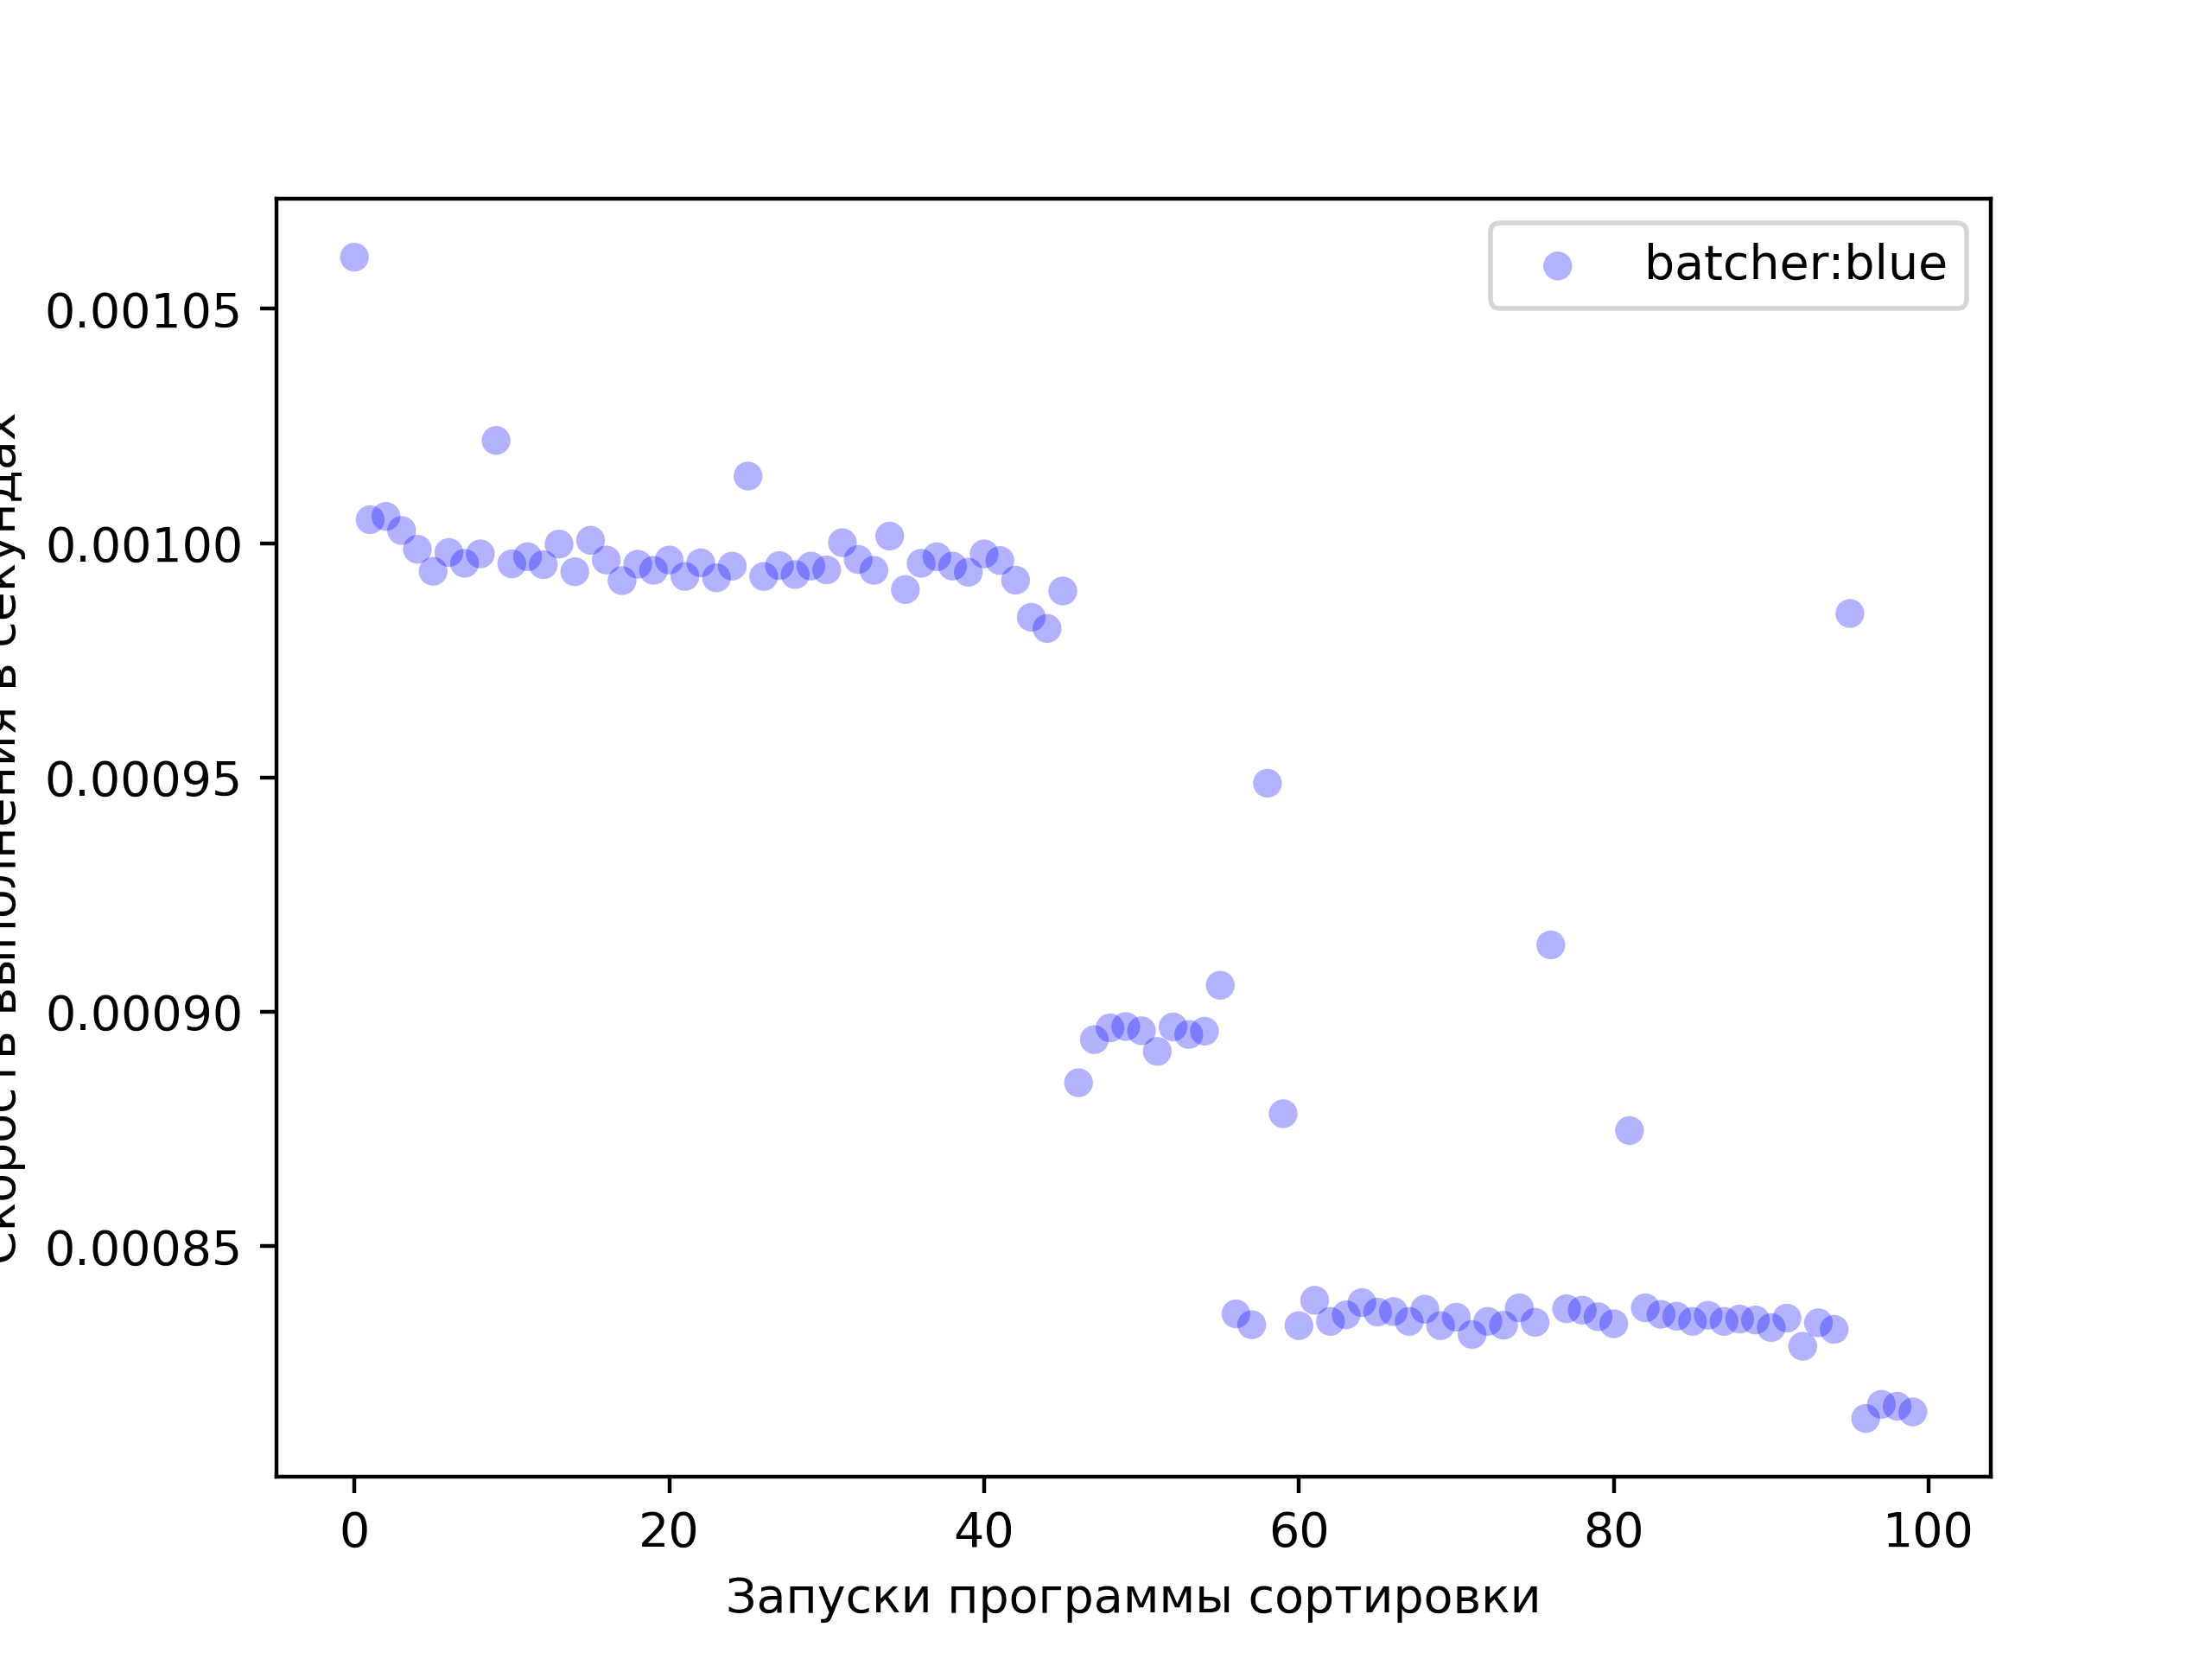
\includegraphics[width=0.9\textwidth]{./plots/batcher_speed.png}
    \caption{График сортировки Бэтчера}
\end{figure}


\textit{Скорость выполнения сортировки на основе приоритетных очередей в сравнении с сортировкой Бэтчера}

\begin{figure}[H]
    \centering
    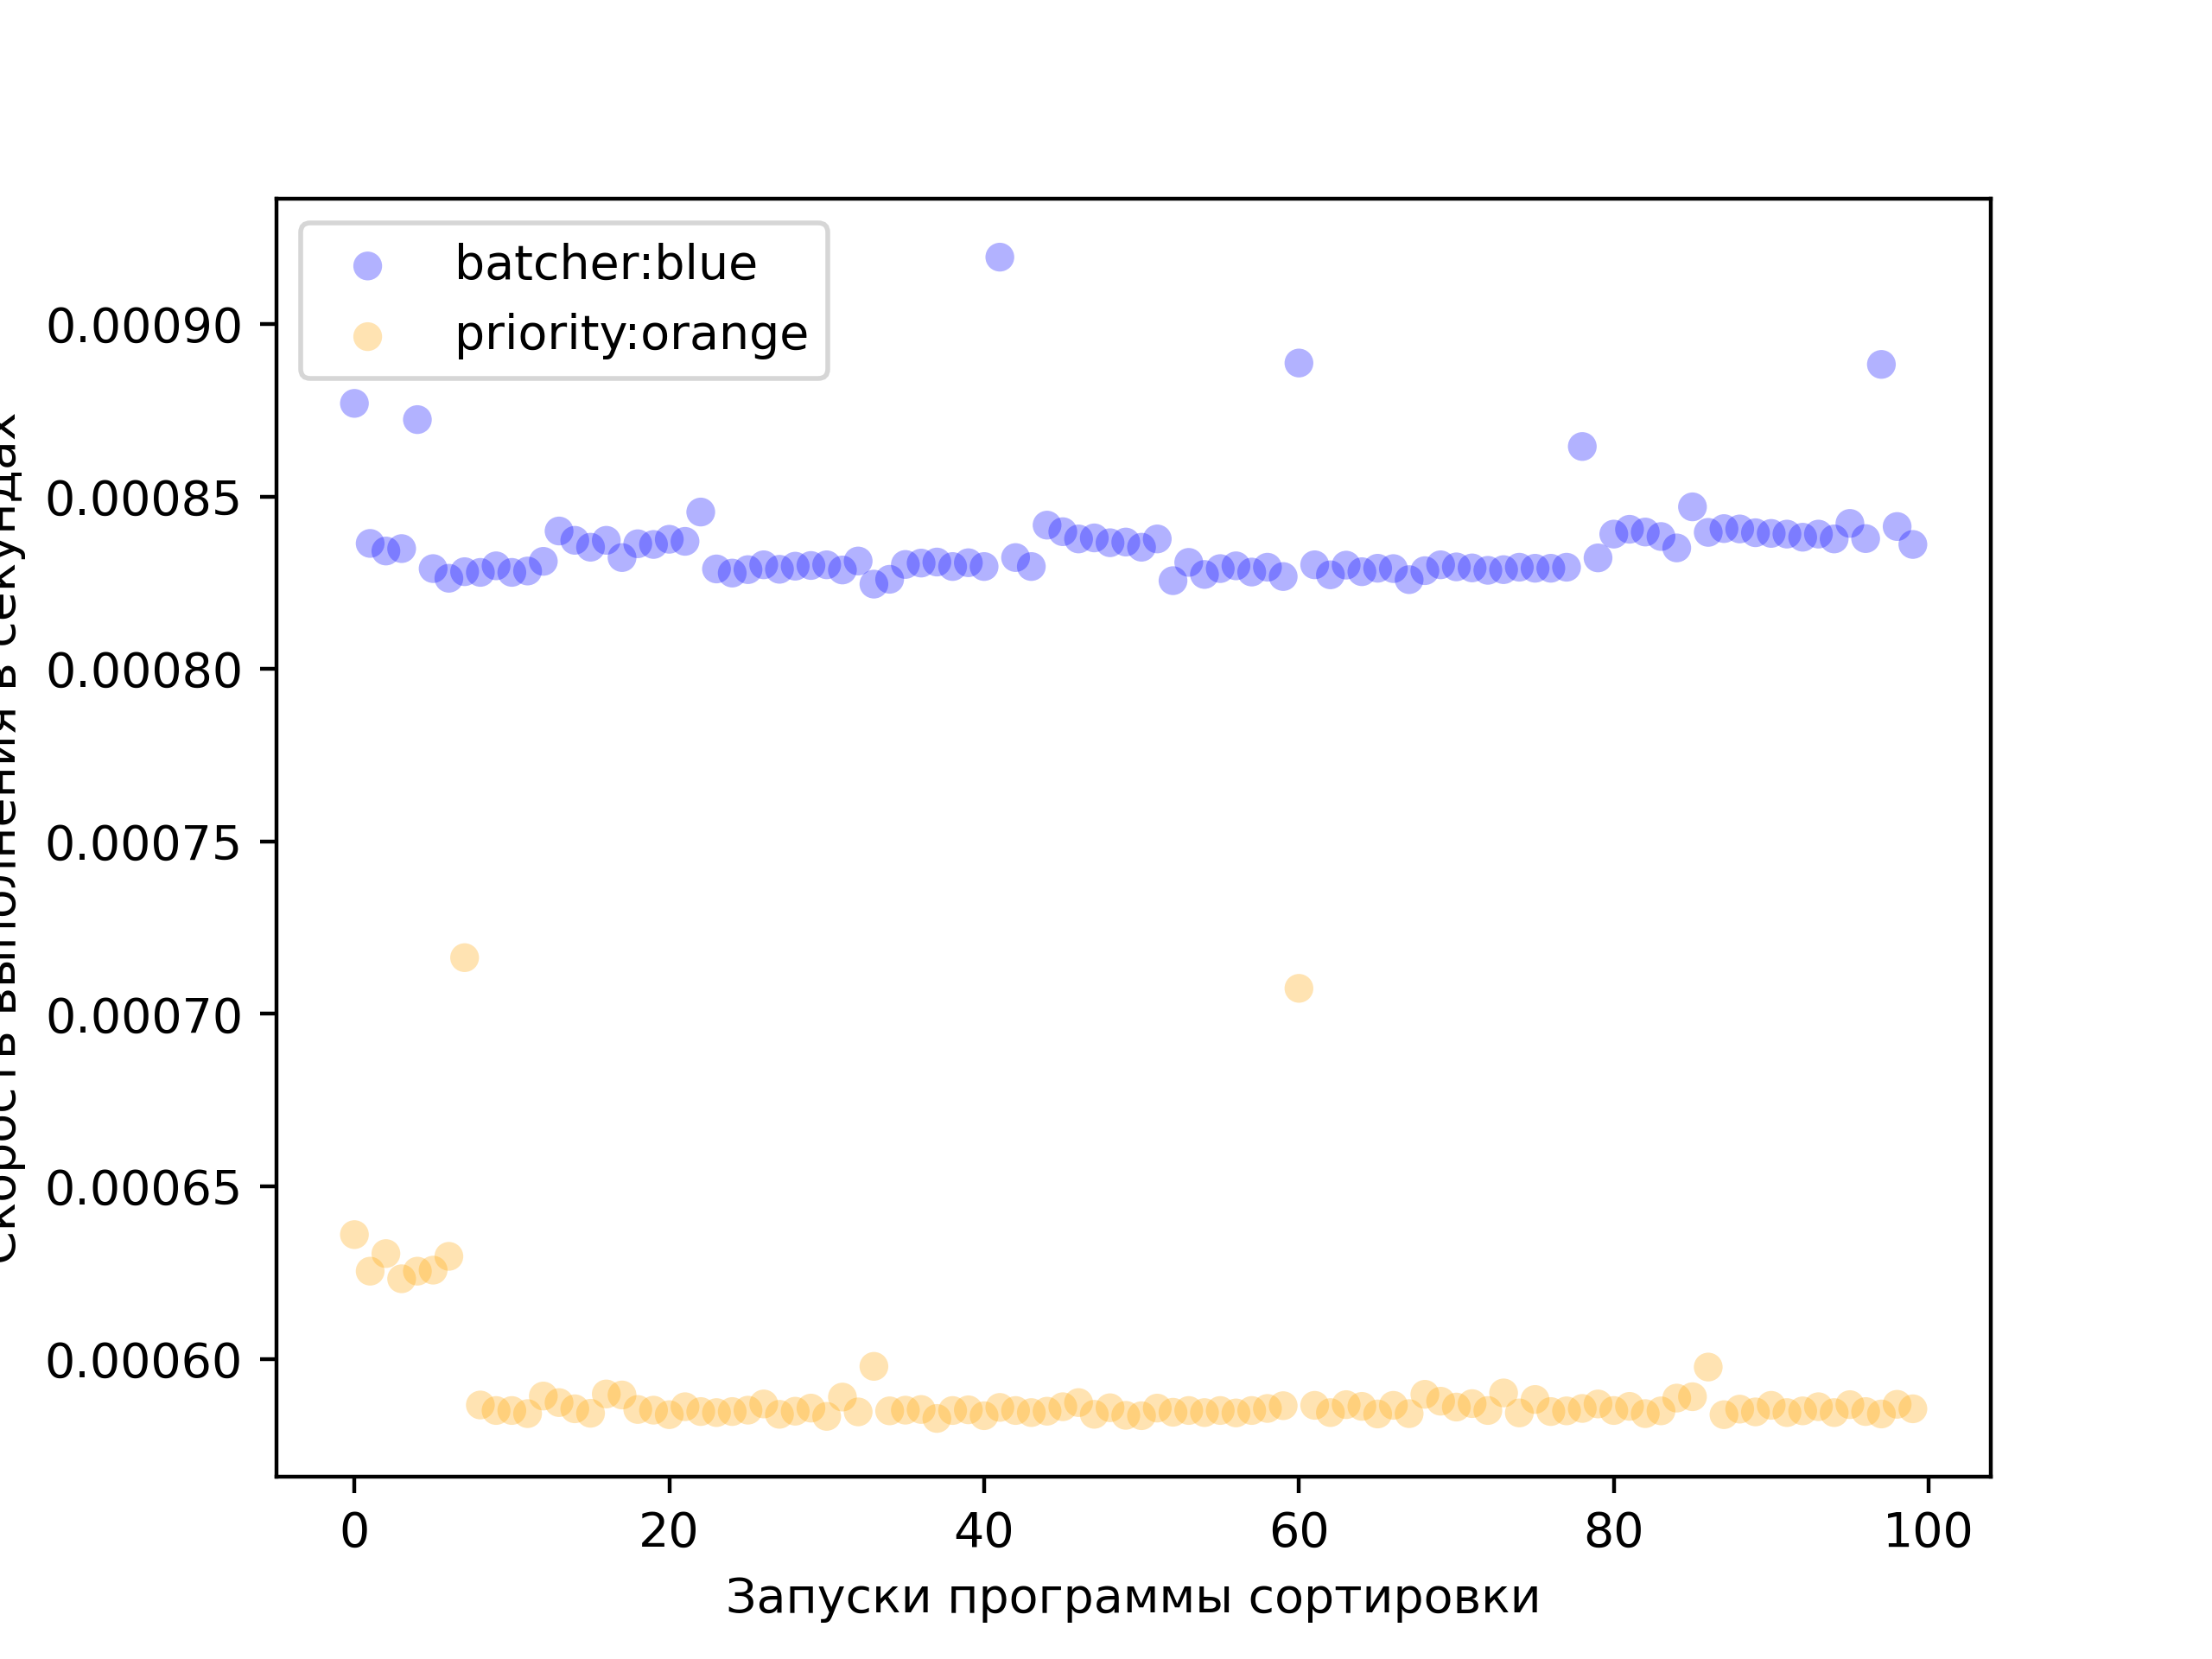
\includegraphics[width=0.9\textwidth]{./plots/priority_speed.png}
    \caption{График сортировки Приоритетных очередей}
\end{figure}



\textit{Скорость выполнения сортировки Пирамидой в сравнении с остальными двумя сортировками}

\begin{figure}[H]
    \centering
    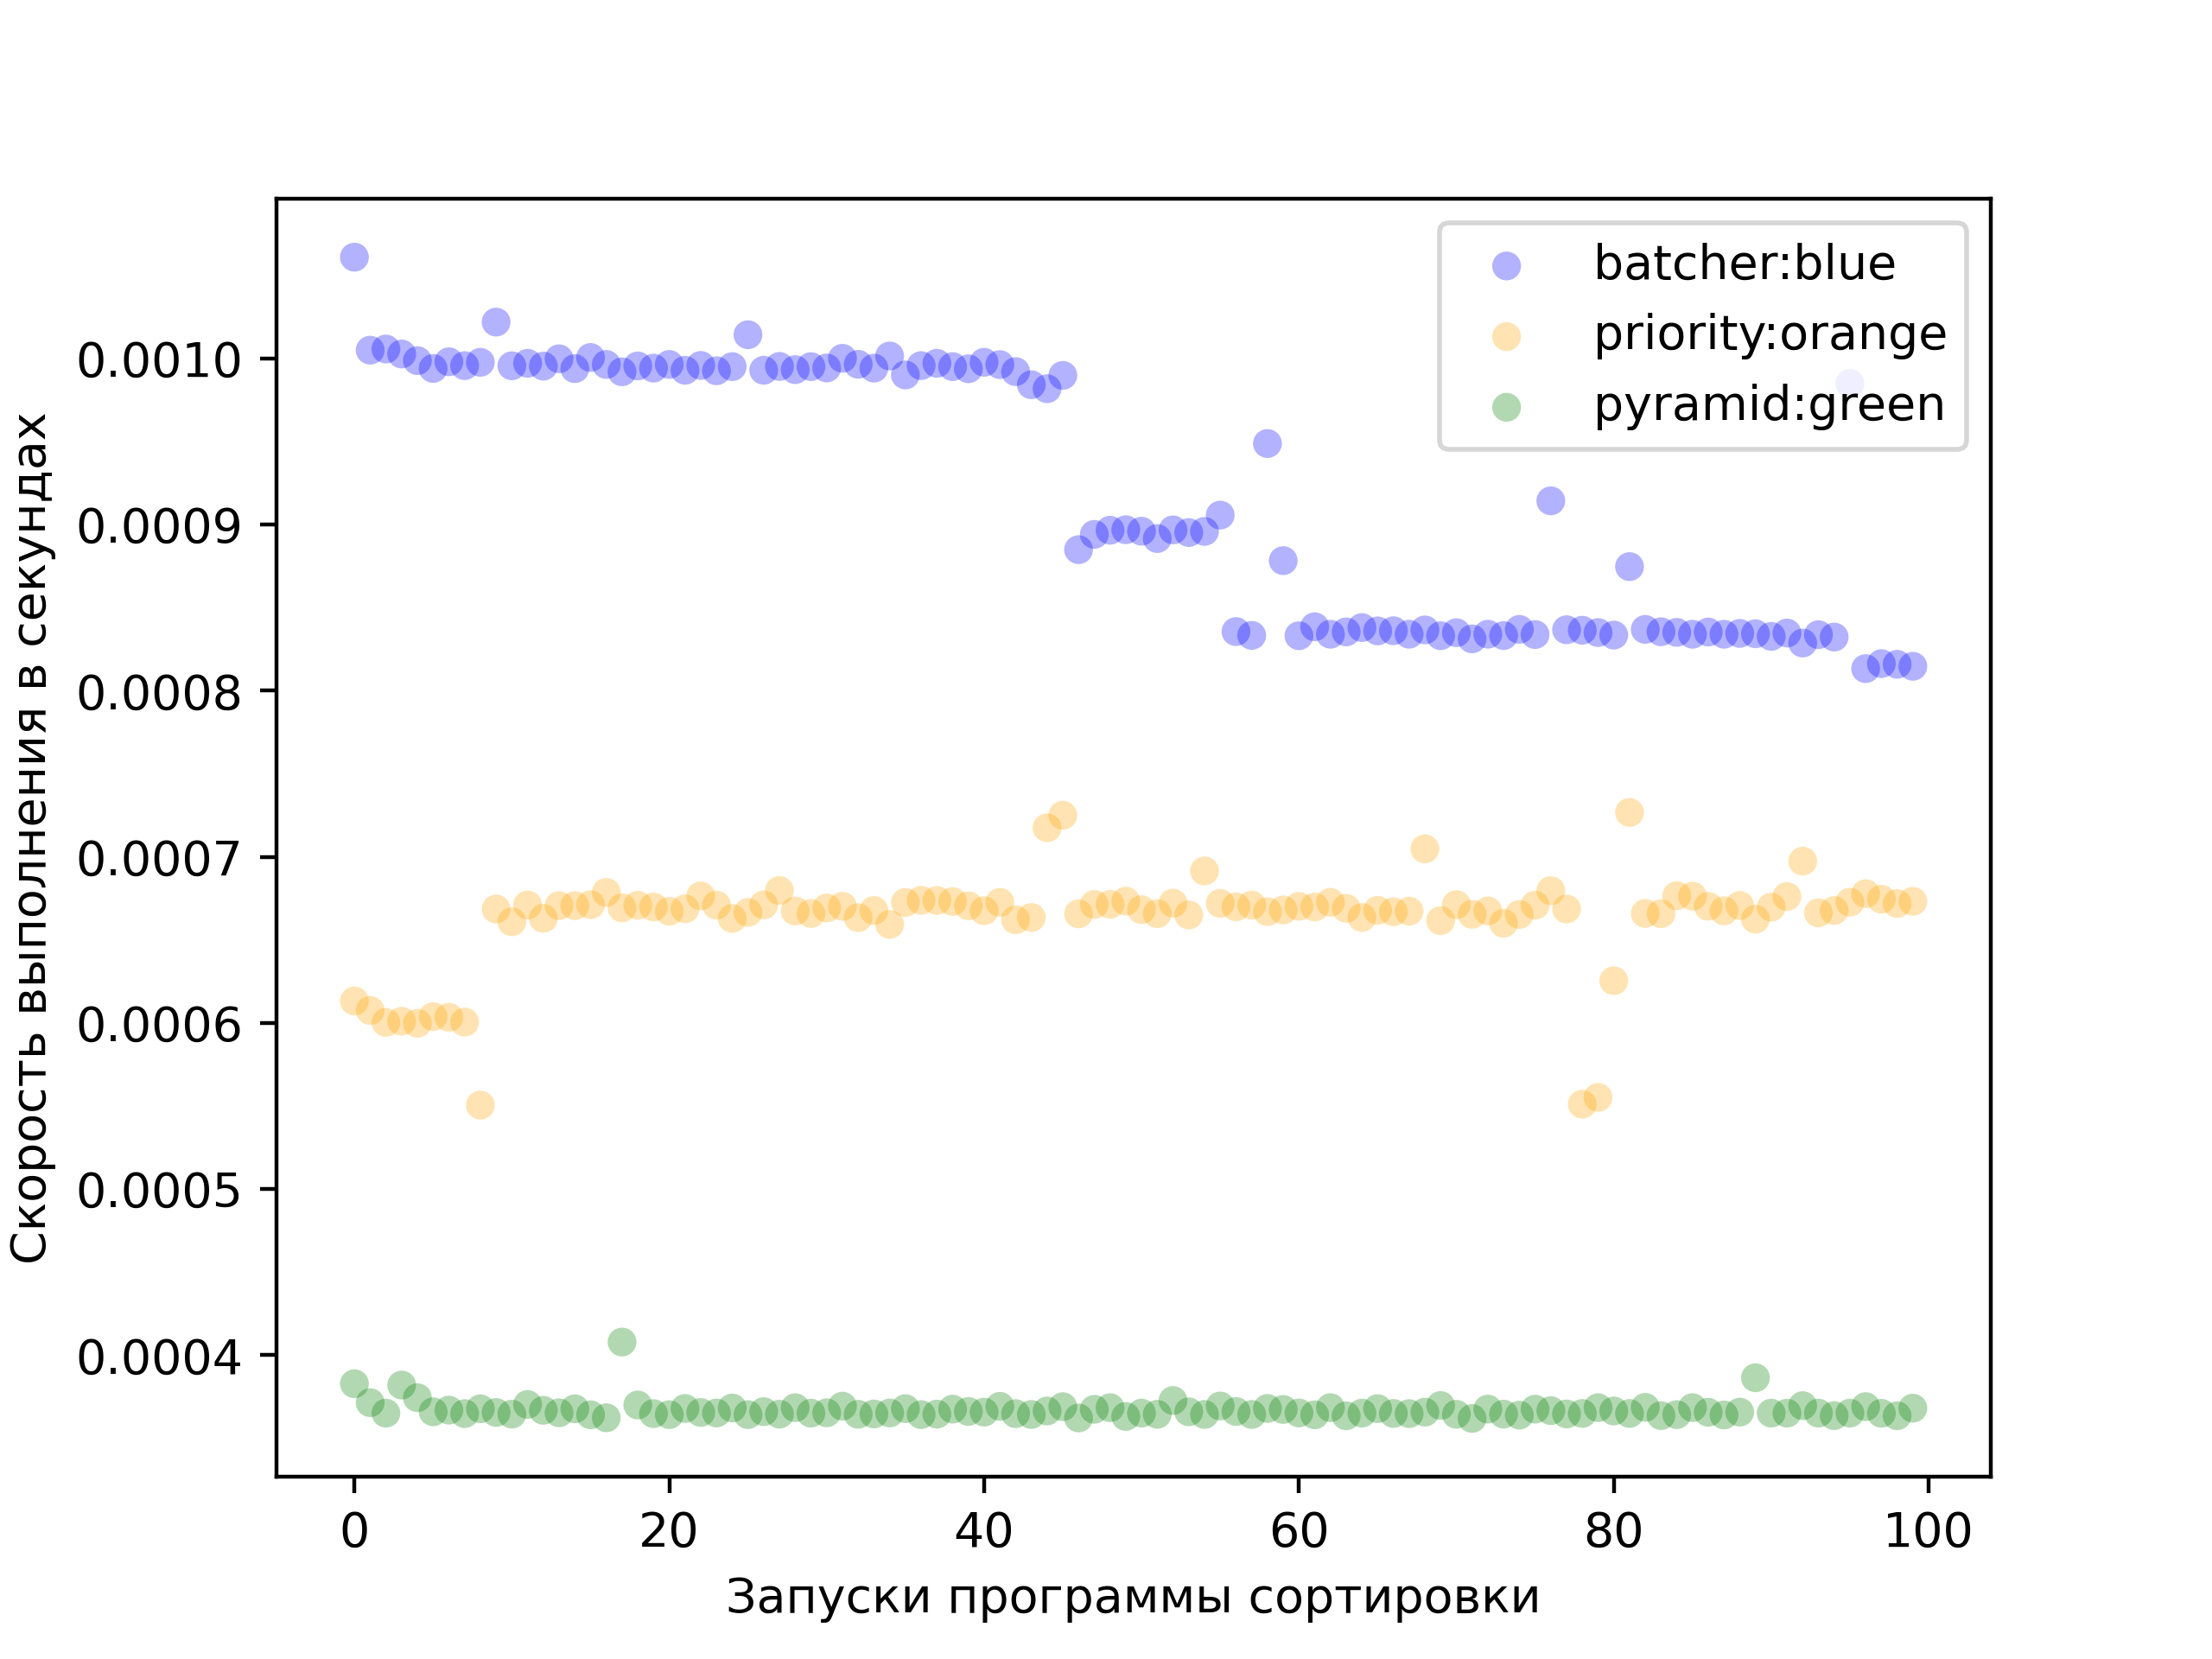
\includegraphics[width=0.9\textwidth]{./plots/bitonic_speed.png}
    \caption{График сортировки Пирамидой}
\end{figure}








\subsection{Потребление памяти алгоритмов}






Программа 3 импортирует 3 подпрограммы сортировки и строит графики для трех алгоритмов сортировки.

По оси х Запуски программ

По оси у Потребление памяти

\textbf{Исходный код Программы 3}

\lstinputlisting[language = python]{../memory_usage.py}


\newpage
\textbf{Таким образом были построены графики:}

\textit{Потребление памяти сортировки Бэтчера}

\begin{figure}[H]
    \centering
    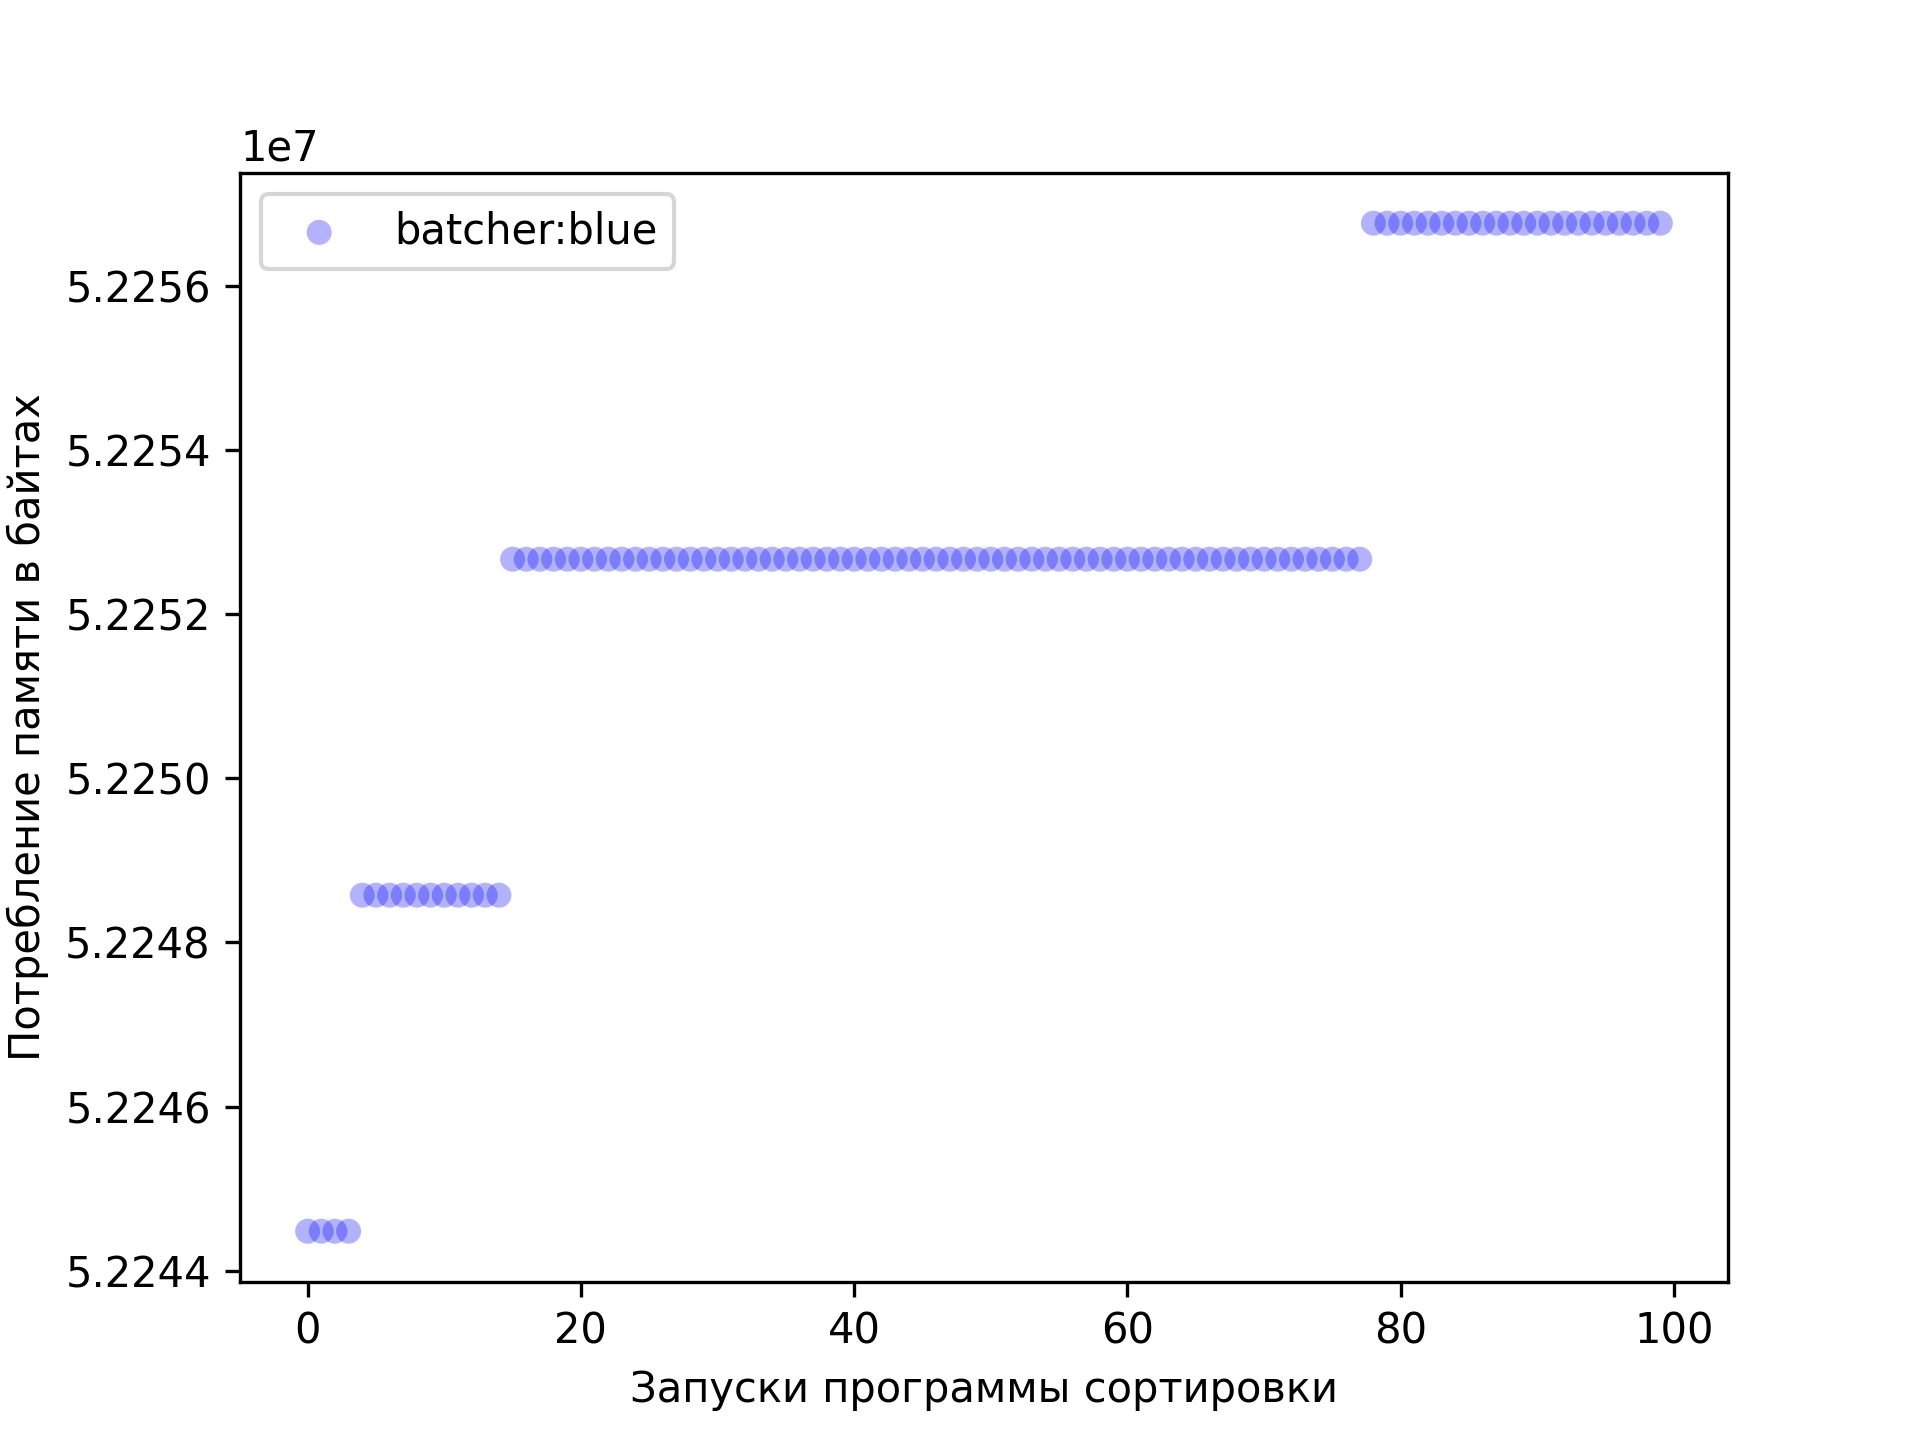
\includegraphics[width=0.9\textwidth]{./plots/batcher_memory.png}
    \caption{График сортировки Бэтчера}
\end{figure}


\textit{Потребление памяти сортировки на основе приоритетных очередей в сравнении с сортировкой Бэтчера}

\begin{figure}[H]
    \centering
    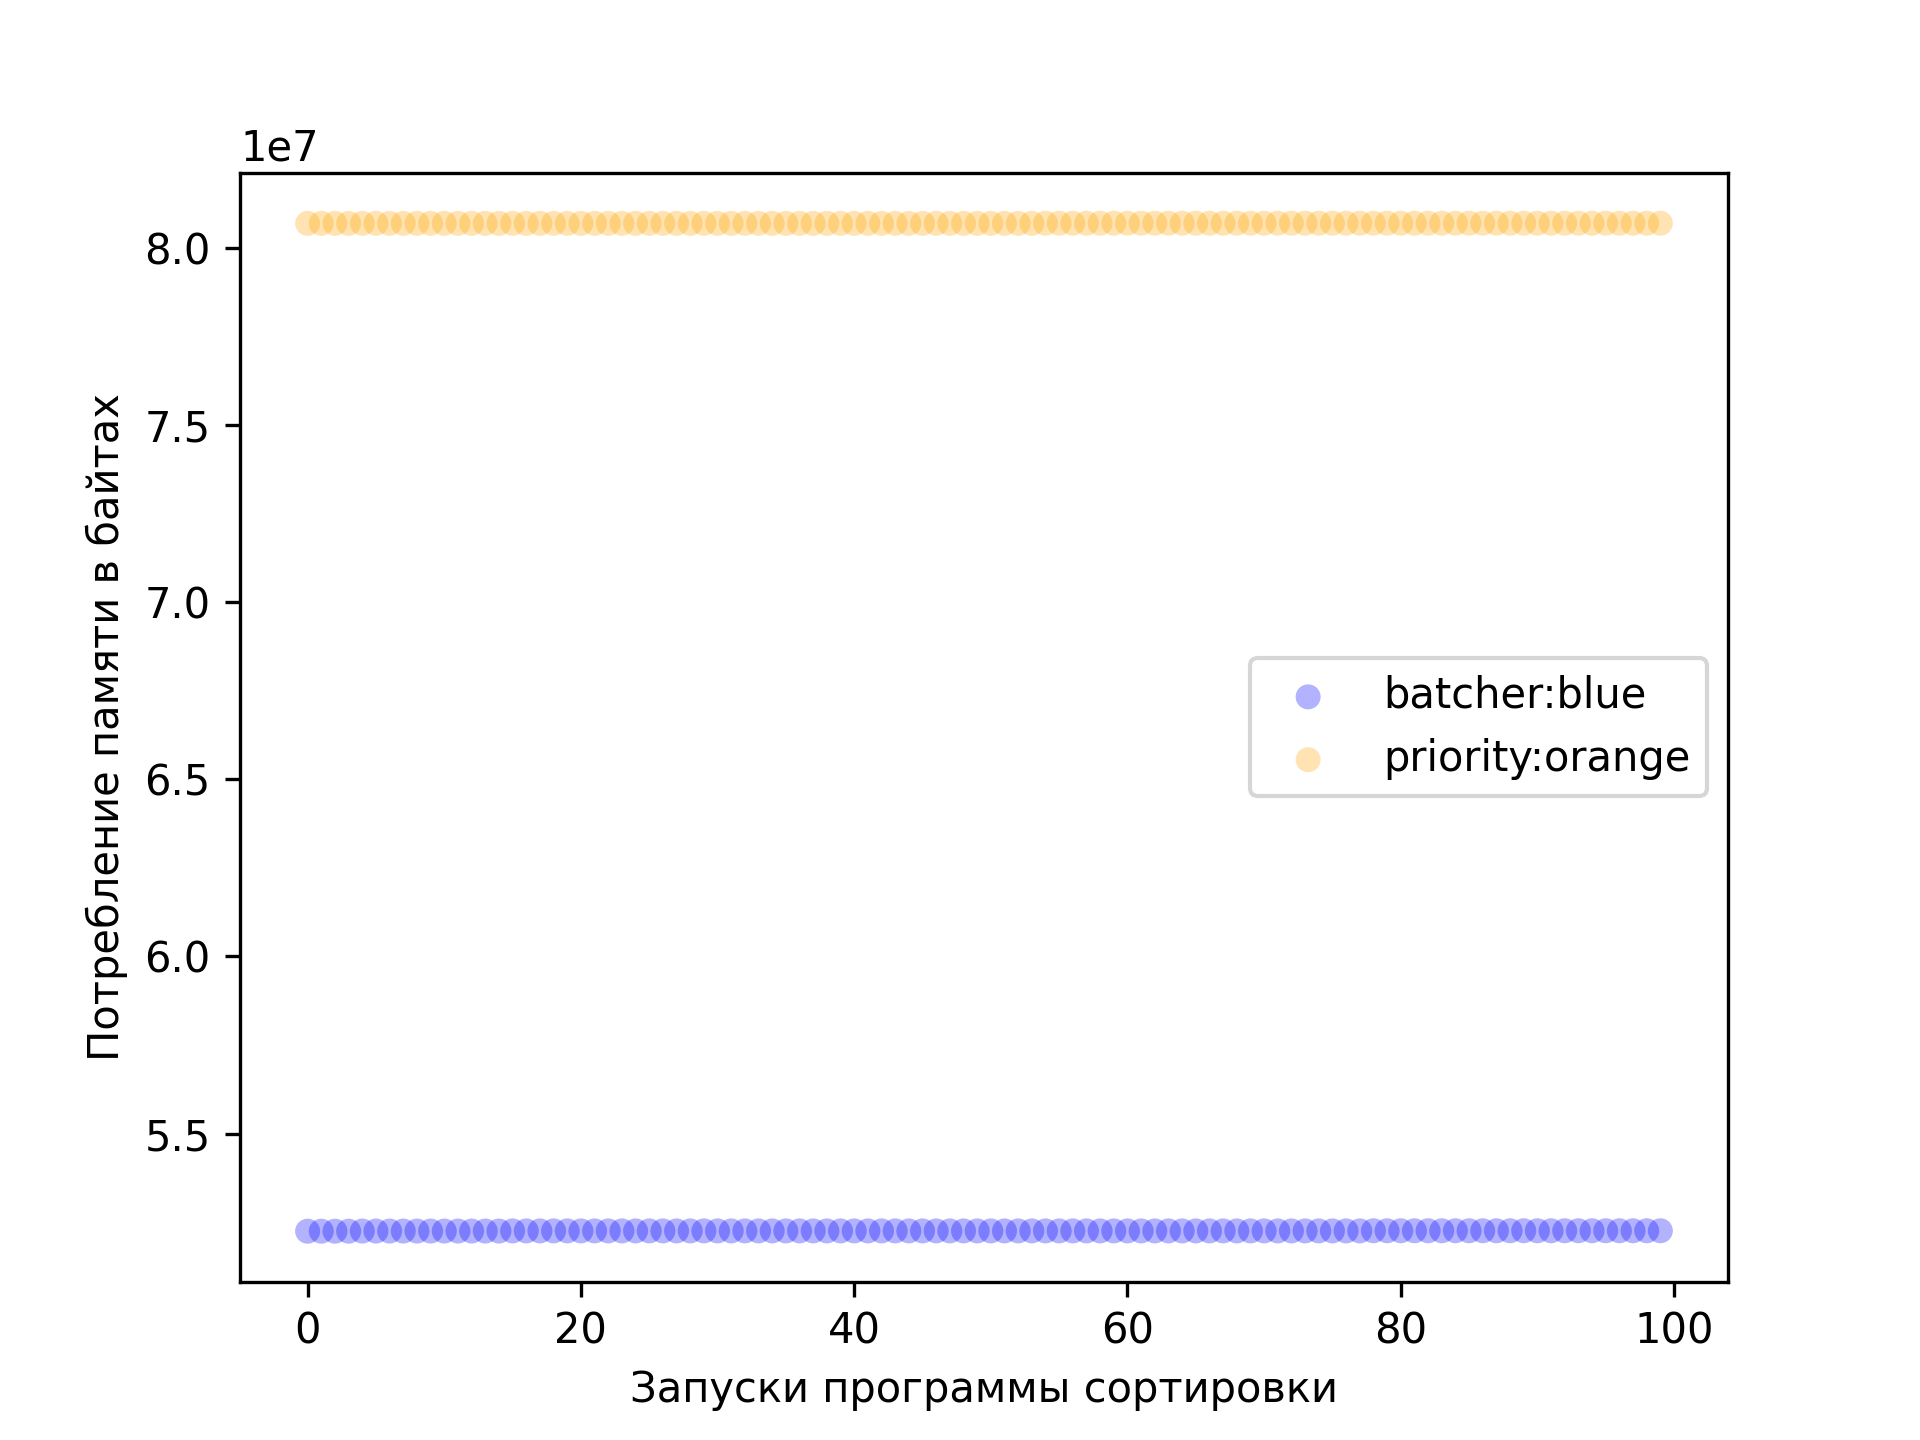
\includegraphics[width=0.9\textwidth]{./plots/priority_memory.png}
    \caption{График сортировки Приоритетных очередей}
\end{figure}



\textit{Потребление памяти сортировки Пирамидой в сравнении с остальными двумя сортировками}

\begin{figure}[H]
    \centering
    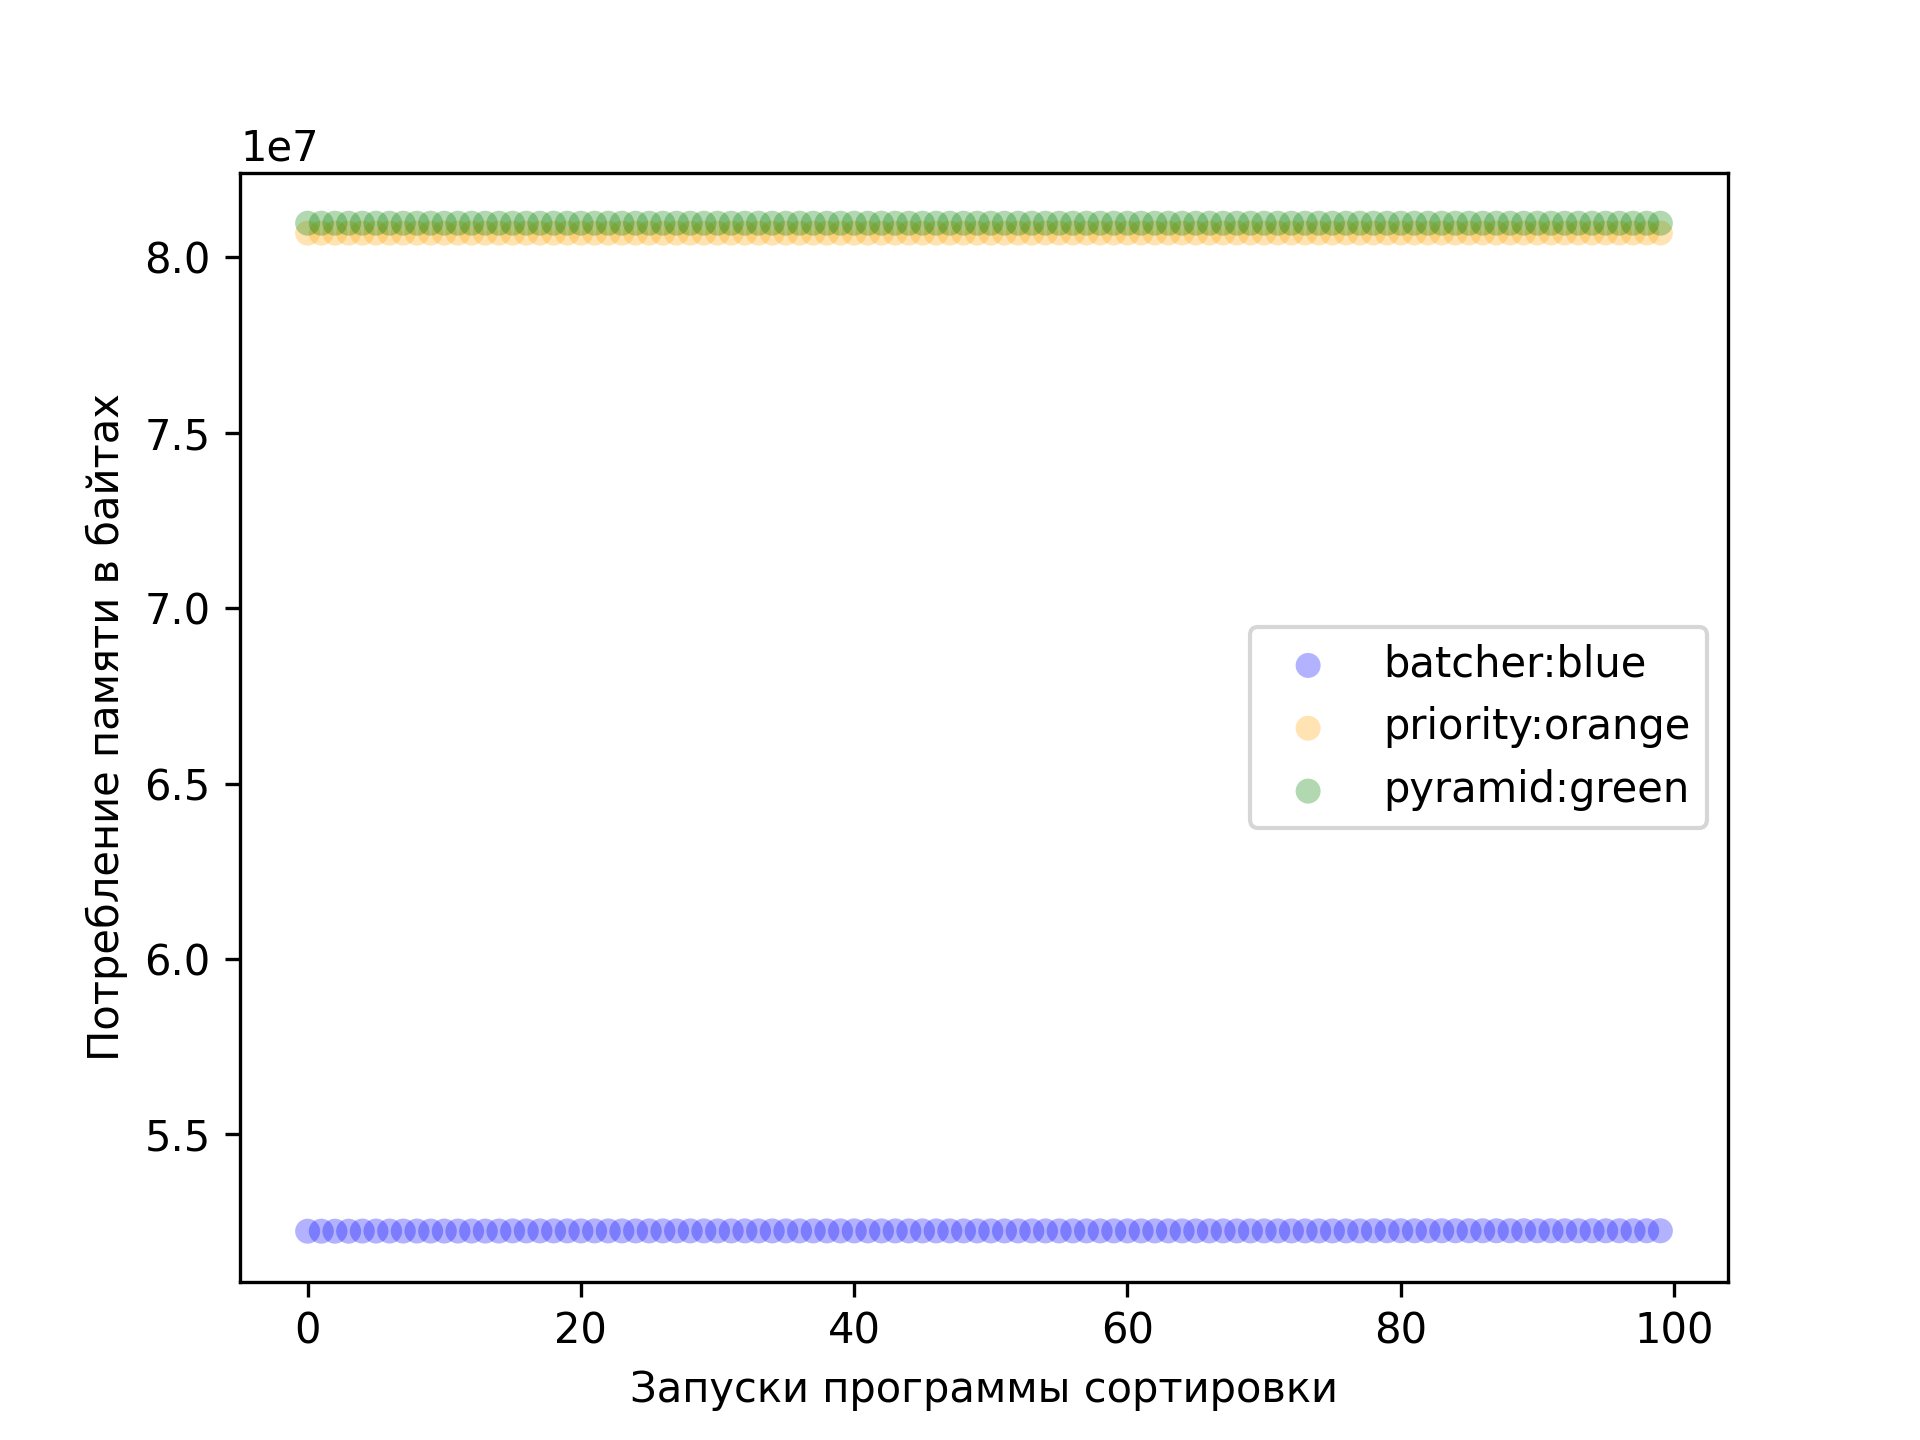
\includegraphics[width=1\textwidth]{./plots/bitonic_memory.png}
    \caption{График сортировки Пирамидой}
\end{figure}

\section{Выводы по трем алгоритмам}





























% \begin{table}[H]\centering\caption{batcher sort}\begin{tabular}{|c|c|c|}\hline Запуск программы & Скорость выполнения   & Потребление памяти \\ \hline 1                & 0.0008890000026440248 & 20086784           \\ \hline 2                & 0.0008505000005243346 & 20086784           \\ \hline 3                & 0.0008888000011211261 & 20086784           \\ \hline 4                & 0.0008426999993389472 & 20086784           \\ \hline 5                & 0.0008421999955317006 & 20086784           \\ \hline 6                & 0.0008430000016232952 & 20086784           \\ \hline 7                & 0.0008448000007774681 & 20086784           \\ \hline 8                & 0.0008440000092377886 & 20086784           \\ \hline 9                & 0.0008452999900327995 & 20086784           \\ \hline 10               & 0.0008441999962087721 & 20086784           \\ \hline 11               & 0.0008420999947702512 & 20086784           \\ \hline 12               & 0.0008587999909650534 & 20086784           \\ \hline 13               & 0.000836799998069182  & 20086784           \\ \hline 14               & 0.0008390000002691522 & 20086784           \\ \hline 15               & 0.0008393000025535002 & 20086784           \\ \hline 16               & 0.0008424000116065145 & 20086784           \\ \hline 17               & 0.0008411999879172072 & 20086784           \\ \hline 18               & 0.0008405999979004264 & 20090880           \\ \hline 19               & 0.0008417999924859032 & 20090880           \\ \hline 20               & 0.0008437000069534406 & 20090880           \\ \hline 21               & 0.0008435000054305419 & 20090880           \\ \hline 22               & 0.0008436999924015254 & 20090880           \\ \hline 23               & 0.0008428000001003966 & 20090880           \\ \hline 24               & 0.0008422000100836158 & 20090880           \\ \hline 25               & 0.0008414000039920211 & 20090880           \\ \hline 26               & 0.0008418999932473525 & 20090880           \\ \hline 27               & 0.0008421999955317006 & 20090880           \\ \hline 28               & 0.0008429000008618459 & 20090880           \\ \hline 29               & 0.0008436000061919913 & 20090880           \\ \hline 30               & 0.0009122999908868223 & 20094976           \\ \hline 31               & 0.0008470000029774383 & 20094976           \\ \hline 32               & 0.0008422999962931499 & 20094976           \\ \hline 33               & 0.0008432000031461939 & 20094976           \\ \hline 34               & 0.0008437000069534406 & 20094976           \\ \hline 35               & 0.0008432000031461939 & 20094976           \\ \hline 36               & 0.0008431000023847446 & 20094976           \\ \hline 37               & 0.0008440999954473227 & 20094976           \\ \hline 38               & 0.0008423999970545992 & 20094976           \\ \hline 39               & 0.0008410000009462237 & 20094976           \\ \hline 40               & 0.0008455000061076134 & 20094976           \\ \hline\end{tabular}\end{table}



\end{document}
